\section{Organización general}

El procesador implementa un pipeline \emph{in-order} de cinco etapas. La
arquitectura mantiene el orden del programa: una instrucción más nueva no puede
adelantarse a una anterior ni modificar el estado arquitectónico antes que
ella. El solapamiento cambia cuántas instrucciones están activas al mismo
tiempo, pero no la semántica secuencial.

El recorrido de las cinco etapas se muestra en la
figura~\ref{fig:pipeline}. Las etapas y sus contratos se desarrollan en
\doc{architecture/cpu/cpu_pipeline.md}{Pipeline de la CPU}; el detalle de
señales, muxes y caminos de datos se encuentra en
\doc{architecture/cpu/datapath.md}{Datapath}.

\section{Modelo temporal y ocupación}

En un ciclo efectivo, cada etapa trabaja sobre una instrucción distinta y los
registros interetapa capturan el resultado de la etapa anterior. La
tabla~\ref{tab:ocupacion} muestra la ocupación ideal de cinco instrucciones
independientes, sin hazards ni cambios de flujo. Cada instrucción avanza una
etapa por ciclo y el pipeline alcanza a tener cinco instrucciones activas.

\begin{table}[H]
  \centering
  \small
  \setlength{\tabcolsep}{3pt}
  \begin{tabular}{l*{9}{c}}
    \toprule
    \textbf{Instrucción} & C1 & C2 & C3 & C4 & C5 & C6 & C7 & C8 & C9 \\
    \midrule
    I1 & IF & ID & EX & MEM & WB & --- & --- & --- & --- \\
    I2 & --- & IF & ID & EX & MEM & WB & --- & --- & --- \\
    I3 & --- & --- & IF & ID & EX & MEM & WB & --- & --- \\
    I4 & --- & --- & --- & IF & ID & EX & MEM & WB & --- \\
    I5 & --- & --- & --- & --- & IF & ID & EX & MEM & WB \\
    \bottomrule
  \end{tabular}
  \caption{Ocupación ideal de cinco instrucciones independientes. Cada columna
  representa un ciclo efectivo y cada fila una instrucción.}
  \label{tab:ocupacion}
\end{table}

En el régimen ideal, el pipeline entrega una instrucción por ciclo después de
llenarse, por lo que el CPI se aproxima a uno. Las desviaciones tienen causas
concretas:

\begin{itemize}
  \item Una dependencia inmediata \code{load-use} retiene al consumidor e
    inserta una burbuja en \code{ID/EX}. El load avanza y el consumidor
    continúa un ciclo después, cuando el dato ya puede reenviarse a traves de forwarding.
  \item Un branch tomado, \code{JAL} o \code{JALR} se resuelve en EX. El
    redirect invalida las dos instrucciones más jóvenes que ya habían entrado
    al pipeline y produce una penalización de dos ciclos.
  \item Un fault confirmado o un \code{halt} detiene el ingreso de instrucciones
    nuevas. El pipeline se drena para completar solamente las instrucciones
    anteriores que todavía estaban en vuelo.
\end{itemize}

\section{Instruction Fetch (IF)}

La etapa IF inicia el recorrido de cada instrucción. En cada ciclo efectivo
consulta la dirección indicada por el PC global, obtiene una palabra de IMEM y
forma el candidato que el control puede capturar en \code{IF/ID}. La lectura de IMEM es
combinacional: la palabra está disponible dentro del mismo ciclo.

En el recorrido secuencial, IF propone \code{PC + 4} como próximo PC. Si EX
confirma un branch tomado, \code{JAL} o \code{JALR}, el control reemplaza esa
dirección por el destino del redirect y descarta las instrucciones jóvenes que
ya habían sido buscadas.

Los bloques principales de la etapa son:

\begin{itemize}
  \item \textbf{\code{PC}:} conserva la dirección de la búsqueda actual y se
    actualiza cuando el control habilita un nuevo ciclo de ejecución.
  \item \textbf{\code{PC Adder}:} calcula la continuación secuencial sumando
    cuatro bytes al PC actual.
  \item \textbf{\code{Next PC MUX}:} selecciona entre \code{PC + 4} y el
    destino de un redirect producido por EX.
  \item \textbf{\code{PC Update Control}:} determina si el PC debe actualizarse
    y qué entrada del multiplexor debe utilizarse.
  \item \textbf{\code{Instruction Memory}:} entrega la palabra de 32 bits
    almacenada en la dirección indicada por el PC.
  \item \textbf{\code{Fetch Fault Check}:} comprueba la alineación, el rango
    de IMEM y la pertenencia de los cuatro bytes a la imagen cargada.
  \item \textbf{\code{IF/ID Input Logic}:} combina la instrucción, su PC y el
    resultado de la validación para formar los campos de entrada de \code{IF/ID}.
  \item \textbf{\code{IF/ID Update Control}:} traduce la acción del pipeline en
    una captura, una retención o una invalidación del registro interetapa.
  \item \textbf{Registro \code{IF/ID}:} conserva la instrucción o el candidato
    de fault de fetch hasta que ID pueda procesarlo.
\end{itemize}

Antes de aceptar el resultado como instrucción, IF valida la búsqueda:

\begin{itemize}
  \item el PC debe estar alineado a cuatro bytes;
  \item los cuatro bytes deben pertenecer a la capacidad de IMEM;
  \item los cuatro bytes deben pertenecer a la imagen confirmada.
\end{itemize}

Si la validación falla, IF no produce una instrucción activa: genera un
\emph{candidato de fault de fetch}. El candidato conserva el PC y la causa, y
se transporta por \code{IF/ID}. La confirmación arquitectónica ocurre en ID,
después de respetar el orden de las instrucciones anteriores. Este mecanismo se
describe en \doc{architecture/session/faults_and_termination.md}{Faults,
redirects y terminación}.

El registro \code{IF/ID} conserva cinco campos: \code{valid}, \code{pc},
\code{instruction}, \code{fetch_fault_valid} y
\code{fetch_fault_cause}. En un estado legal, \code{valid} y
\code{fetch_fault_valid} no están activos simultáneamente. La
figura~\ref{fig:etapa-if} muestra el recorrido completo de la etapa.

\begin{figure}[H]
  \centering
  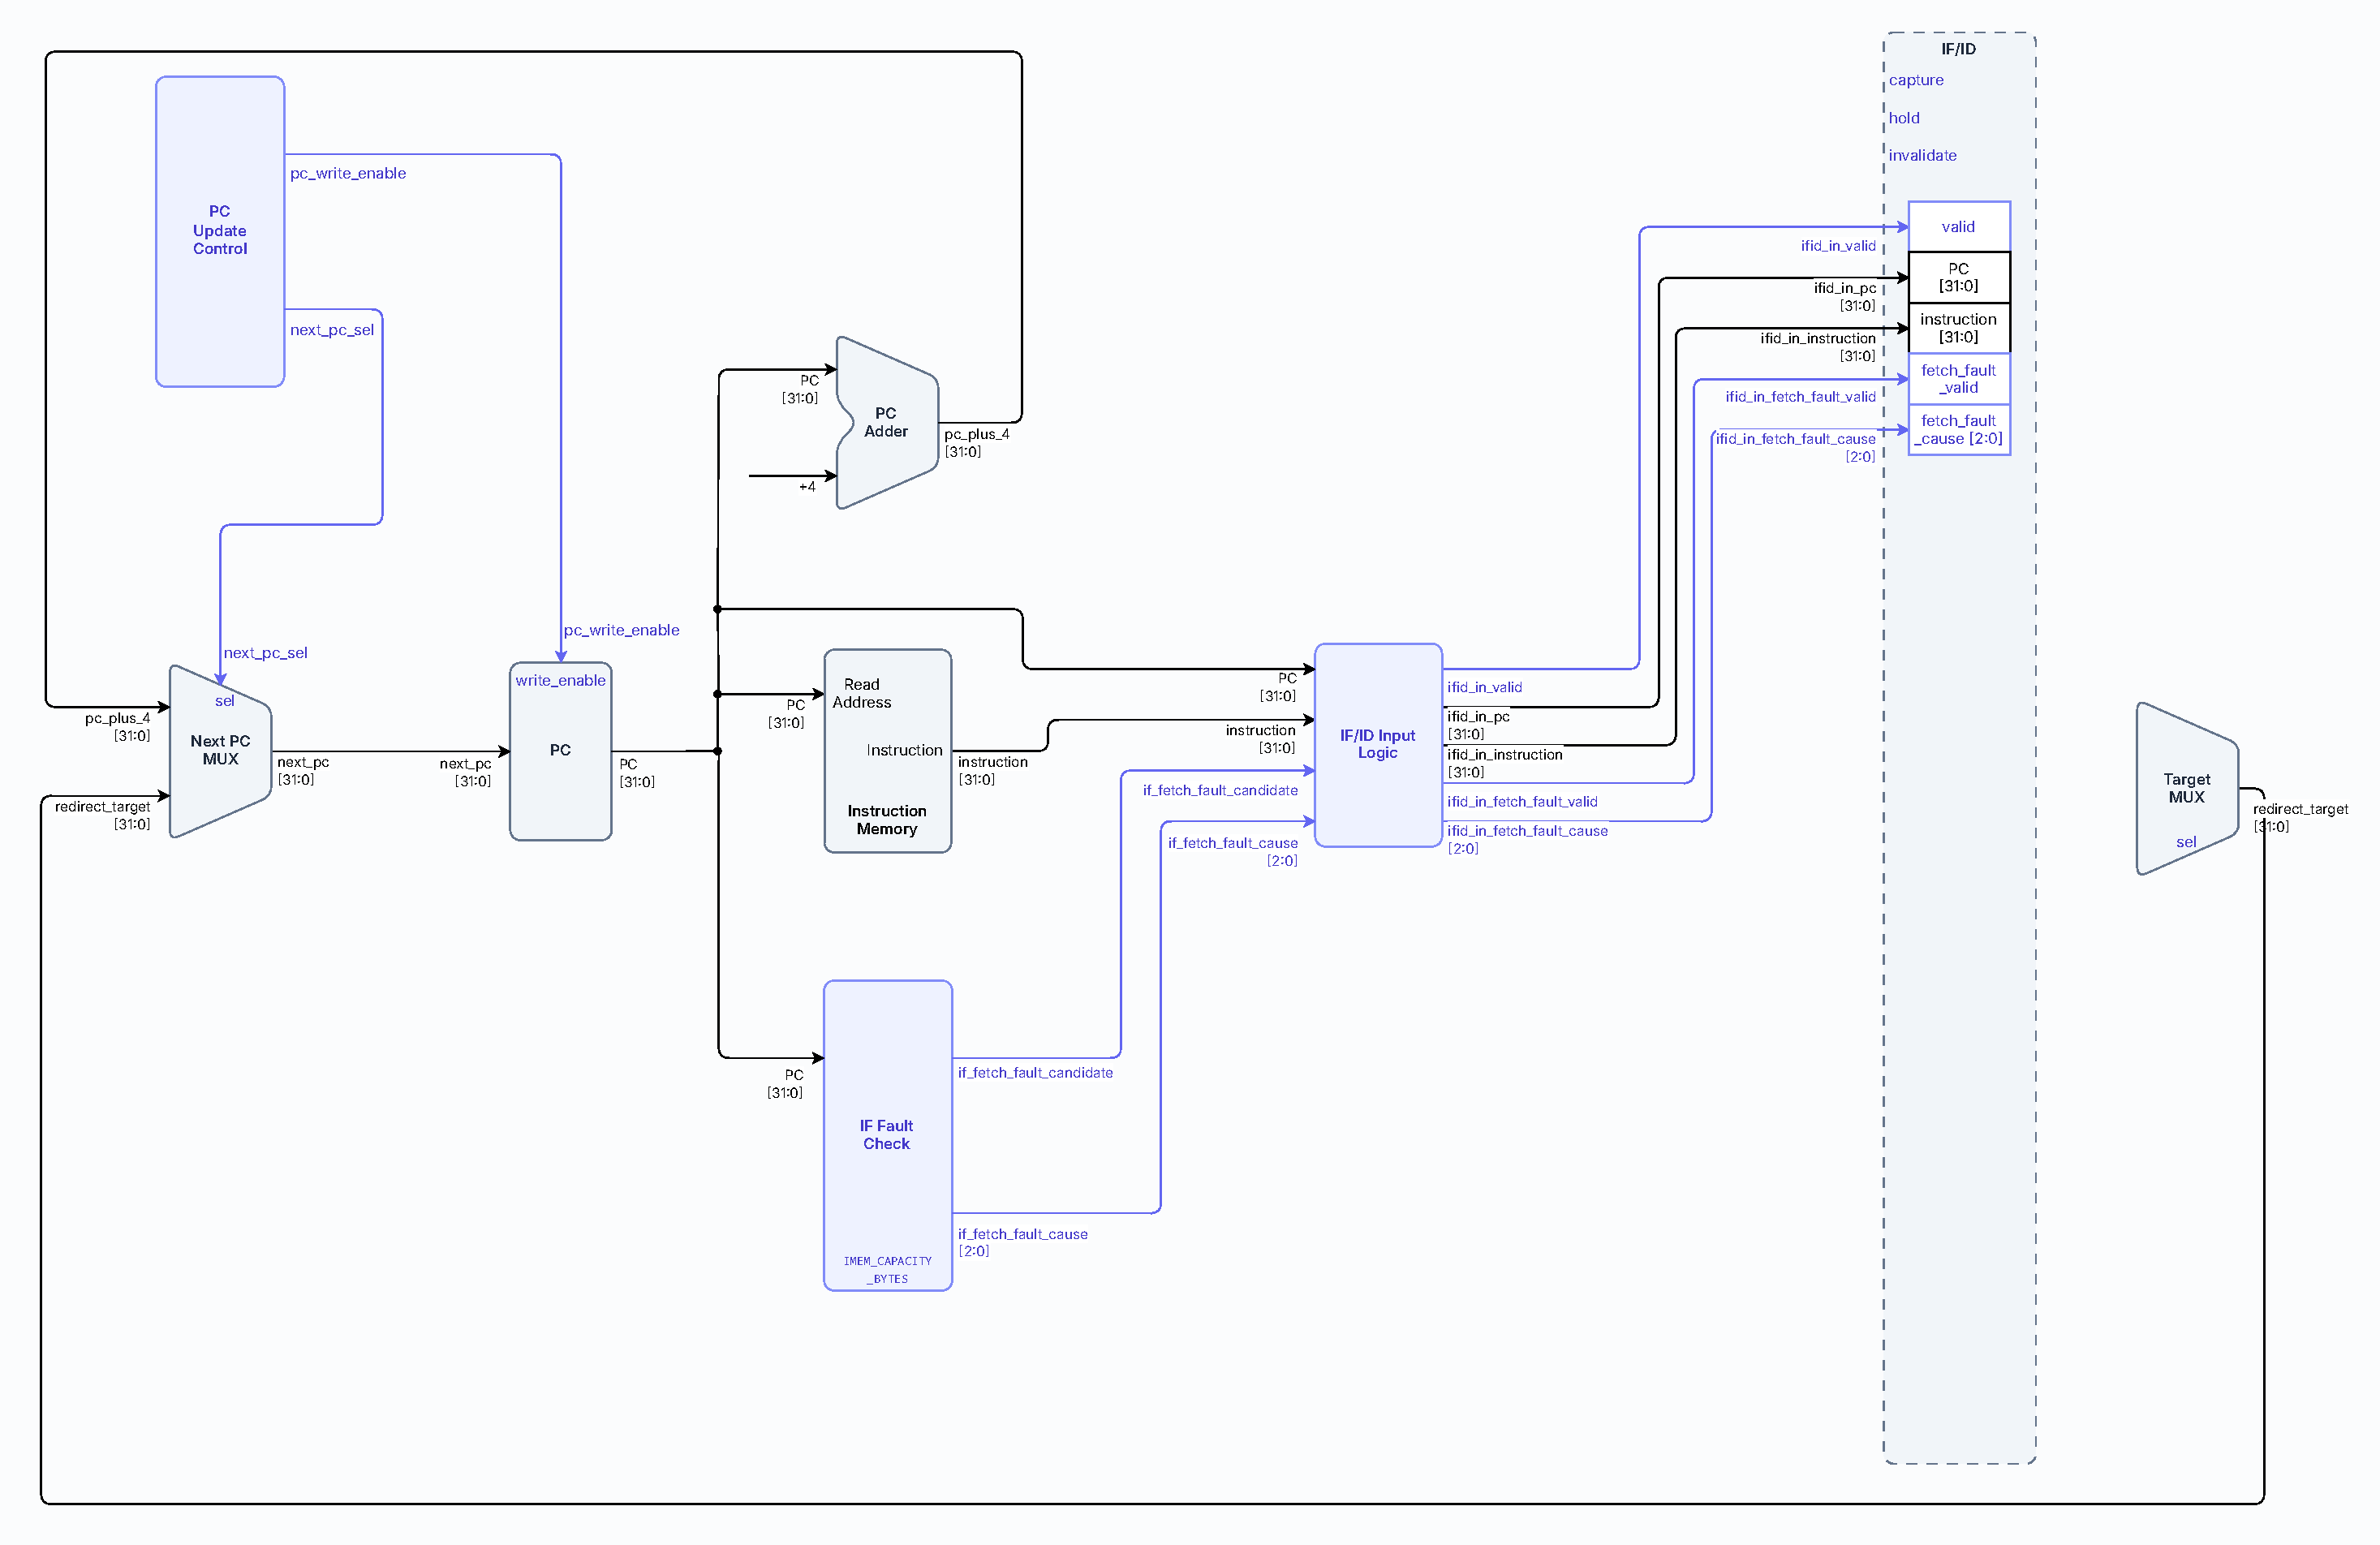
\includegraphics[width=0.95\textwidth]{if-normal.pdf}
  \caption{Recorrido de IF: PC, adder, Instruction Memory, comprobador de
  fetch e IF/ID.}
  \label{fig:etapa-if}
\end{figure}

\section{Instruction Decode (ID)}

La etapa ID recibe desde \code{IF/ID} la instrucción y su PC. En paralelo,
comprueba si la codificación es válida, obtiene los operandos, genera el
inmediato y prepara las señales que EX, MEM y WB necesitarán más adelante.
También resuelve las dependencias que pueden detectarse en esta etapa. El
resultado de ese procesamiento se captura en \code{ID/EX} solo cuando la
acción del pipeline permite avanzar.

\subsection{Bloques principales}

Sus bloques principales son:

\begin{itemize}
  \item \textbf{\code{Decoder}:} reconoce las instrucciones de la whitelist y
    genera los controles de ALU, memoria, flujo, selección de resultado y
    escritura.
  \item \textbf{\code{Register File}:} proporciona las dos lecturas de los
    registros fuente y recibe la escritura síncrona de WB; \code{x0} conserva
    siempre el valor cero.
  \item \textbf{\code{Immediate Generator}:} reconstruye y extiende el
    inmediato según el formato I, S, B, U o J de la instrucción.
  \item \textbf{\code{WB Bypass Control}:} detecta si WB escribe efectivamente
    uno de los registros que ID está leyendo en el mismo ciclo.
  \item \textbf{\code{RS1 Bypass MUX}:} selecciona el valor de WB para la
    fuente \code{rs1} cuando hay coincidencia; si no, conserva la lectura del
    banco de registros.
  \item \textbf{\code{RS2 Bypass MUX}:} aplica la misma selección a la fuente
    \code{rs2}, de manera independiente.
  \item \textbf{\code{ID Fault Check}:} combina una codificación ilegal con un
    candidato de fault de fetch para producir el candidato de fault de ID.
  \item \textbf{\code{Load-Use Detector}:} compara el destino de un load en
    \code{ID/EX} con las fuentes que consume la instrucción de \code{IF/ID} y
    solicita una espera cuando la dependencia es inmediata.
  \item \textbf{\code{ID/EX Update Control}:} convierte la acción del pipeline
    en una captura de ID, una retención o una burbuja.
  \item \textbf{Registro \code{ID/EX}:} conserva los operandos, el inmediato,
    el PC y los controles que EX necesita para ejecutar la instrucción.
\end{itemize}

Una vez decodificada la instrucción y aplicados los bypass, ID prepara la
entrada de \code{ID/EX}. Allí quedan registrados los operandos que EX debe
utilizar, el inmediato, el PC, el registro destino y los controles que indican
qué operación realizar, si hay un acceso a memoria y si habrá una escritura en
WB.

Además, ID determina si la instrucción usa realmente \code{rs1} o \code{rs2}.
Esas dos señales (\code{uses_rs1} y \code{uses_rs2}) sirven para que EX y el detector de
\code{load-use} comparen solo las fuentes relevantes. Como se pueden obtener
directamente de la palabra de instrucción, se mantienen como señales
combinacionales y no se almacenan como campos adicionales en \code{ID/EX}.

El banco de registros tiene dos puertos de lectura combinacional y una escritura
síncrona. La escritura solo es efectiva si el ciclo está habilitado, la entrada
de \code{MEM/WB} es válida, \code{reg_write} está activo y el destino no es
\code{x0}. Si ID lee ese mismo registro en el ciclo de writeback, los muxes de
bypass seleccionan directamente el valor de \code{MEM/WB}; así, la captura en
\code{ID/EX} no depende de la semántica de lectura y escritura simultáneas del
almacenamiento físico. La figura~\ref{fig:etapa-id} resume los bloques y caminos
de la etapa.

\begin{figure}[H]
  \centering
  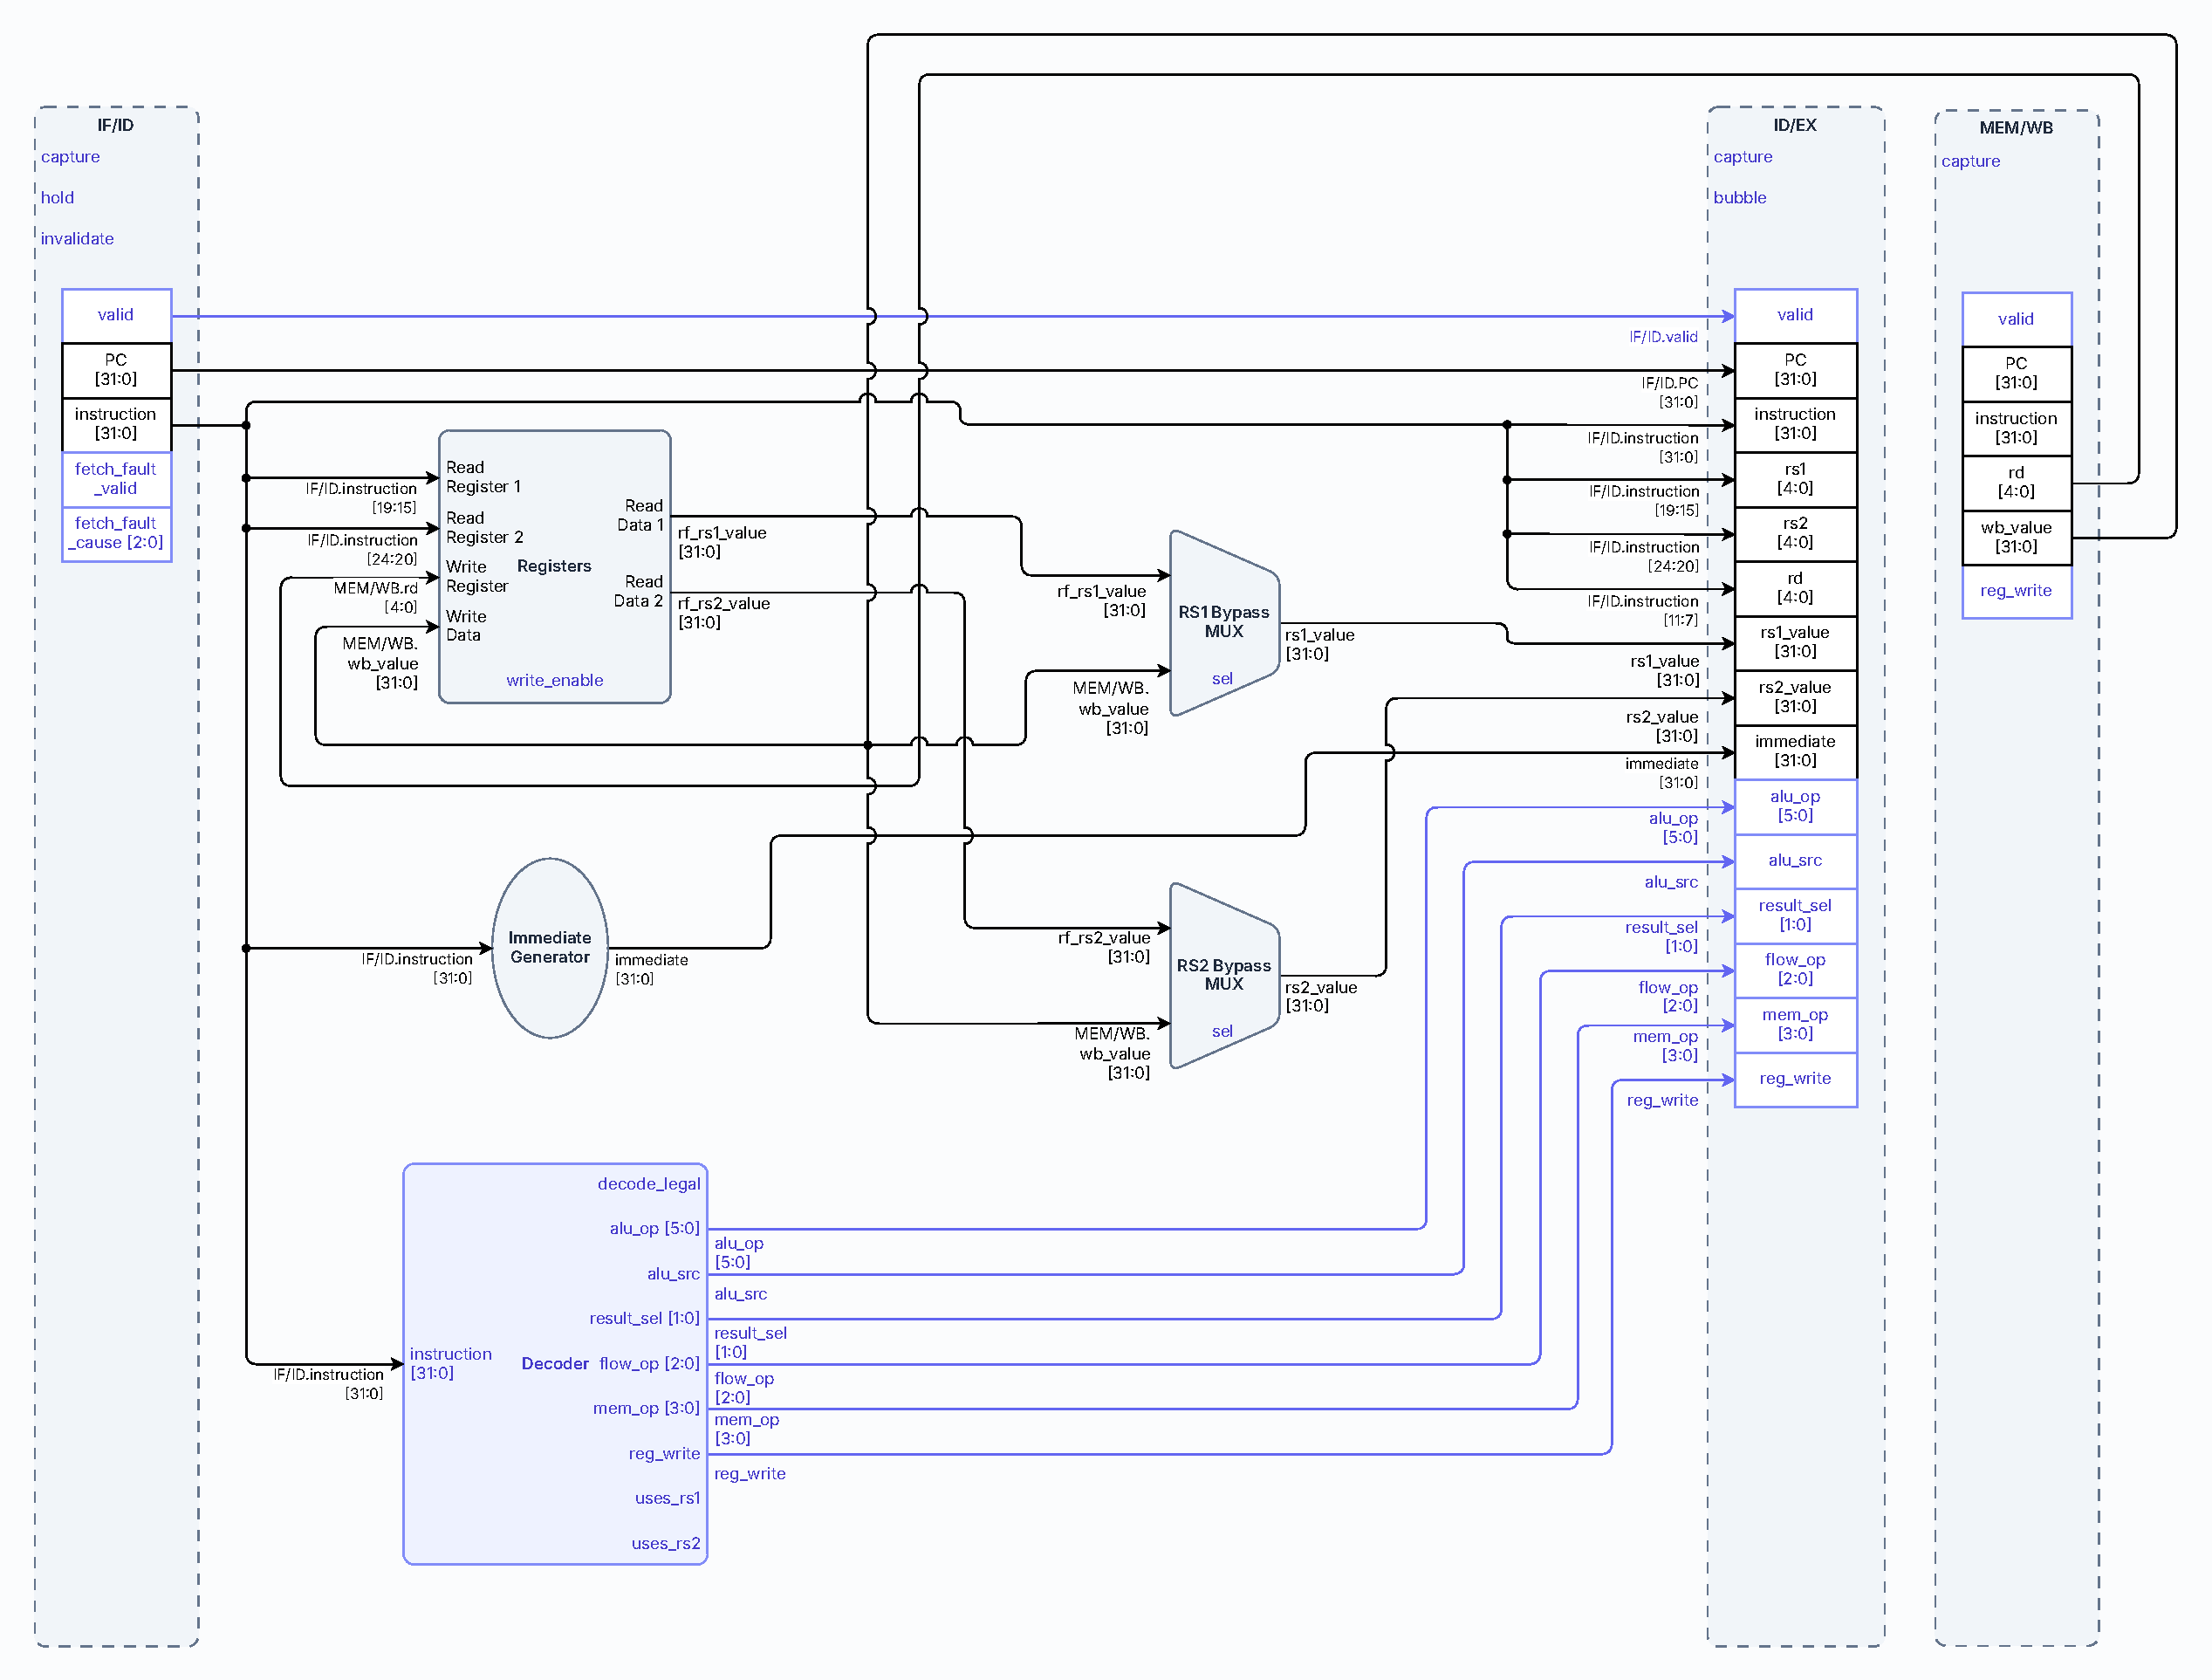
\includegraphics[width=0.95\textwidth]{id-normal.pdf}
  \caption{Recorrido de ID: decoder, banco de registros, generador de
  inmediatos, comprobación de fault y bypass WB$\rightarrow$ID.}
  \label{fig:etapa-id}
\end{figure}

\subsection{Señales de control de ID}

Como resultado de la decodificación, el \code{Decoder} traduce la palabra de
instrucción en un conjunto acotado de señales.
La tabla~\ref{tab:senales-control} resume los códigos que atraviesan
\code{ID/EX} y que después consumen EX, MEM y WB. Los campos
\code{uses_rs1} y \code{uses_rs2} no se almacenan: se calculan a partir de la
instrucción para el forwarding y el detector de load-use.

\begin{table}[H]
  \centering
  \footnotesize
  \setlength{\tabcolsep}{3pt}
  \begin{tabularx}{\textwidth}{L{2.4cm}L{1.0cm}Y}
    \toprule
    \textbf{Señal} & \textbf{Ancho} & \textbf{Valores y significado} \\
    \midrule
    \code{alu_op} & 6 & \code{SLL=0x00}, \code{SRL=0x02}, \code{SRA=0x03},
    \code{ADD=0x20}, \code{SUB=0x22}, \code{AND=0x24}, \code{OR=0x25},
    \code{XOR=0x26}, \code{SLT=0x2A}, \code{SLTU=0x2B}. \\
    \addlinespace
    \code{alu_src} & 1 & \code{0}: segundo operando desde \code{rs2};
    \code{1}: desde el inmediato. \\
    \addlinespace
    \code{result_sel} & 2 & \code{0}: resultado de ALU; \code{1}: inmediato;
    \code{2}: enlace de \code{JAL}/\code{JALR}. \\
    \addlinespace
    \code{flow_op} & 3 & \code{NONE=0}, \code{BEQ=1}, \code{BNE=2},
    \code{JAL=3}, \code{JALR=4}, \code{HALT=5}. \\
    \addlinespace
    \code{mem_op} & 4 & \code{NONE=0}, \code{LB=1}, \code{LH=2}, \code{LW=3},
    \code{LBU=4}, \code{LHU=5}, \code{SB=6}, \code{SH=7}, \code{SW=8}. \\
    \addlinespace
    \code{reg_write} & 1 & \code{0}: no escribe RF; \code{1}: escribe el
    registro \code{rd} si es válido y distinto de \code{x0}. \\
    \bottomrule
  \end{tabularx}
  \caption{Señales de control producidas por el decoder.}
  \label{tab:senales-control}
\end{table}

\section{Execute (EX)}

EX recibe desde \code{ID/EX} una instrucción decodificada, sus operandos base,
el inmediato y las señales de control. Es una etapa combinacional: durante el mismo
ciclo resuelve los operandos, calcula resultados y direcciones, forma los
destinos de salto y genera los candidatos de redirect, \code{halt} y fault.

Sus bloques principales son:

\begin{itemize}
  \item \textbf{\code{Forwarding Unit}:} identifica los productores más
    recientes y selecciona qué valor debe utilizar cada fuente.
  \item \textbf{\code{Forward MUX A} y \code{Forward MUX B}:} producen los
    operandos efectivos \code{rs1_effective} y \code{rs2_effective}.
  \item \textbf{\code{ALU Source MUX}:} elige entre \code{rs2_effective} y el
    inmediato para el segundo operando de la ALU.
  \item \textbf{\code{ALU}:} ejecuta operaciones aritméticas, lógicas,
    comparaciones y desplazamientos, y calcula direcciones efectivas.
  \item \textbf{\code{Link Adder}:} calcula \code{PC + 4}, el valor de enlace
    de \code{JAL} y \code{JALR}.
  \item \textbf{\code{Result MUX}:} selecciona el resultado de ALU, el
    inmediato o el enlace que se conservará como \code{ex_result}.
  \item \textbf{\code{Target Adder} y \code{JALR Adder}:} forman,
    respectivamente, los destinos relativos al PC y los destinos basados en
    \code{rs1}.
  \item \textbf{\code{Clear bit 0} y \code{Target MUX}:} ajustan y seleccionan
    el destino final de un cambio de flujo.
  \item \textbf{\code{Flow Control}:} determina si un branch se toma y genera
    las solicitudes de redirect o el candidato de \code{halt}.
  \item \textbf{\code{EX Fault Check}:} valida accesos a DMEM y destinos de
    control, y produce el candidato de fault propio de EX.
  \item \textbf{\code{EX/MEM Update Control} y registro \code{EX/MEM}:}
    capturan los datos que MEM, WB y Debug todavía necesitan.
\end{itemize}

\subsection{Resolución de operandos}

La unidad de forwarding actúa antes de todos los usos de los operandos. Los
valores efectivos alimentan:

\begin{itemize}
  \item la ALU, para operaciones aritméticas, lógicas, comparaciones y
    desplazamientos;
  \item el cálculo de la dirección efectiva de loads y stores;
  \item la comparación de branches;
  \item la base de \code{JALR};
  \item el sumador de enlace y el cálculo de destinos de \code{JAL}.
\end{itemize}

La figura~\ref{fig:etapa-ex} resume el camino de una operación de registro.

\begin{figure}[H]
  \centering
  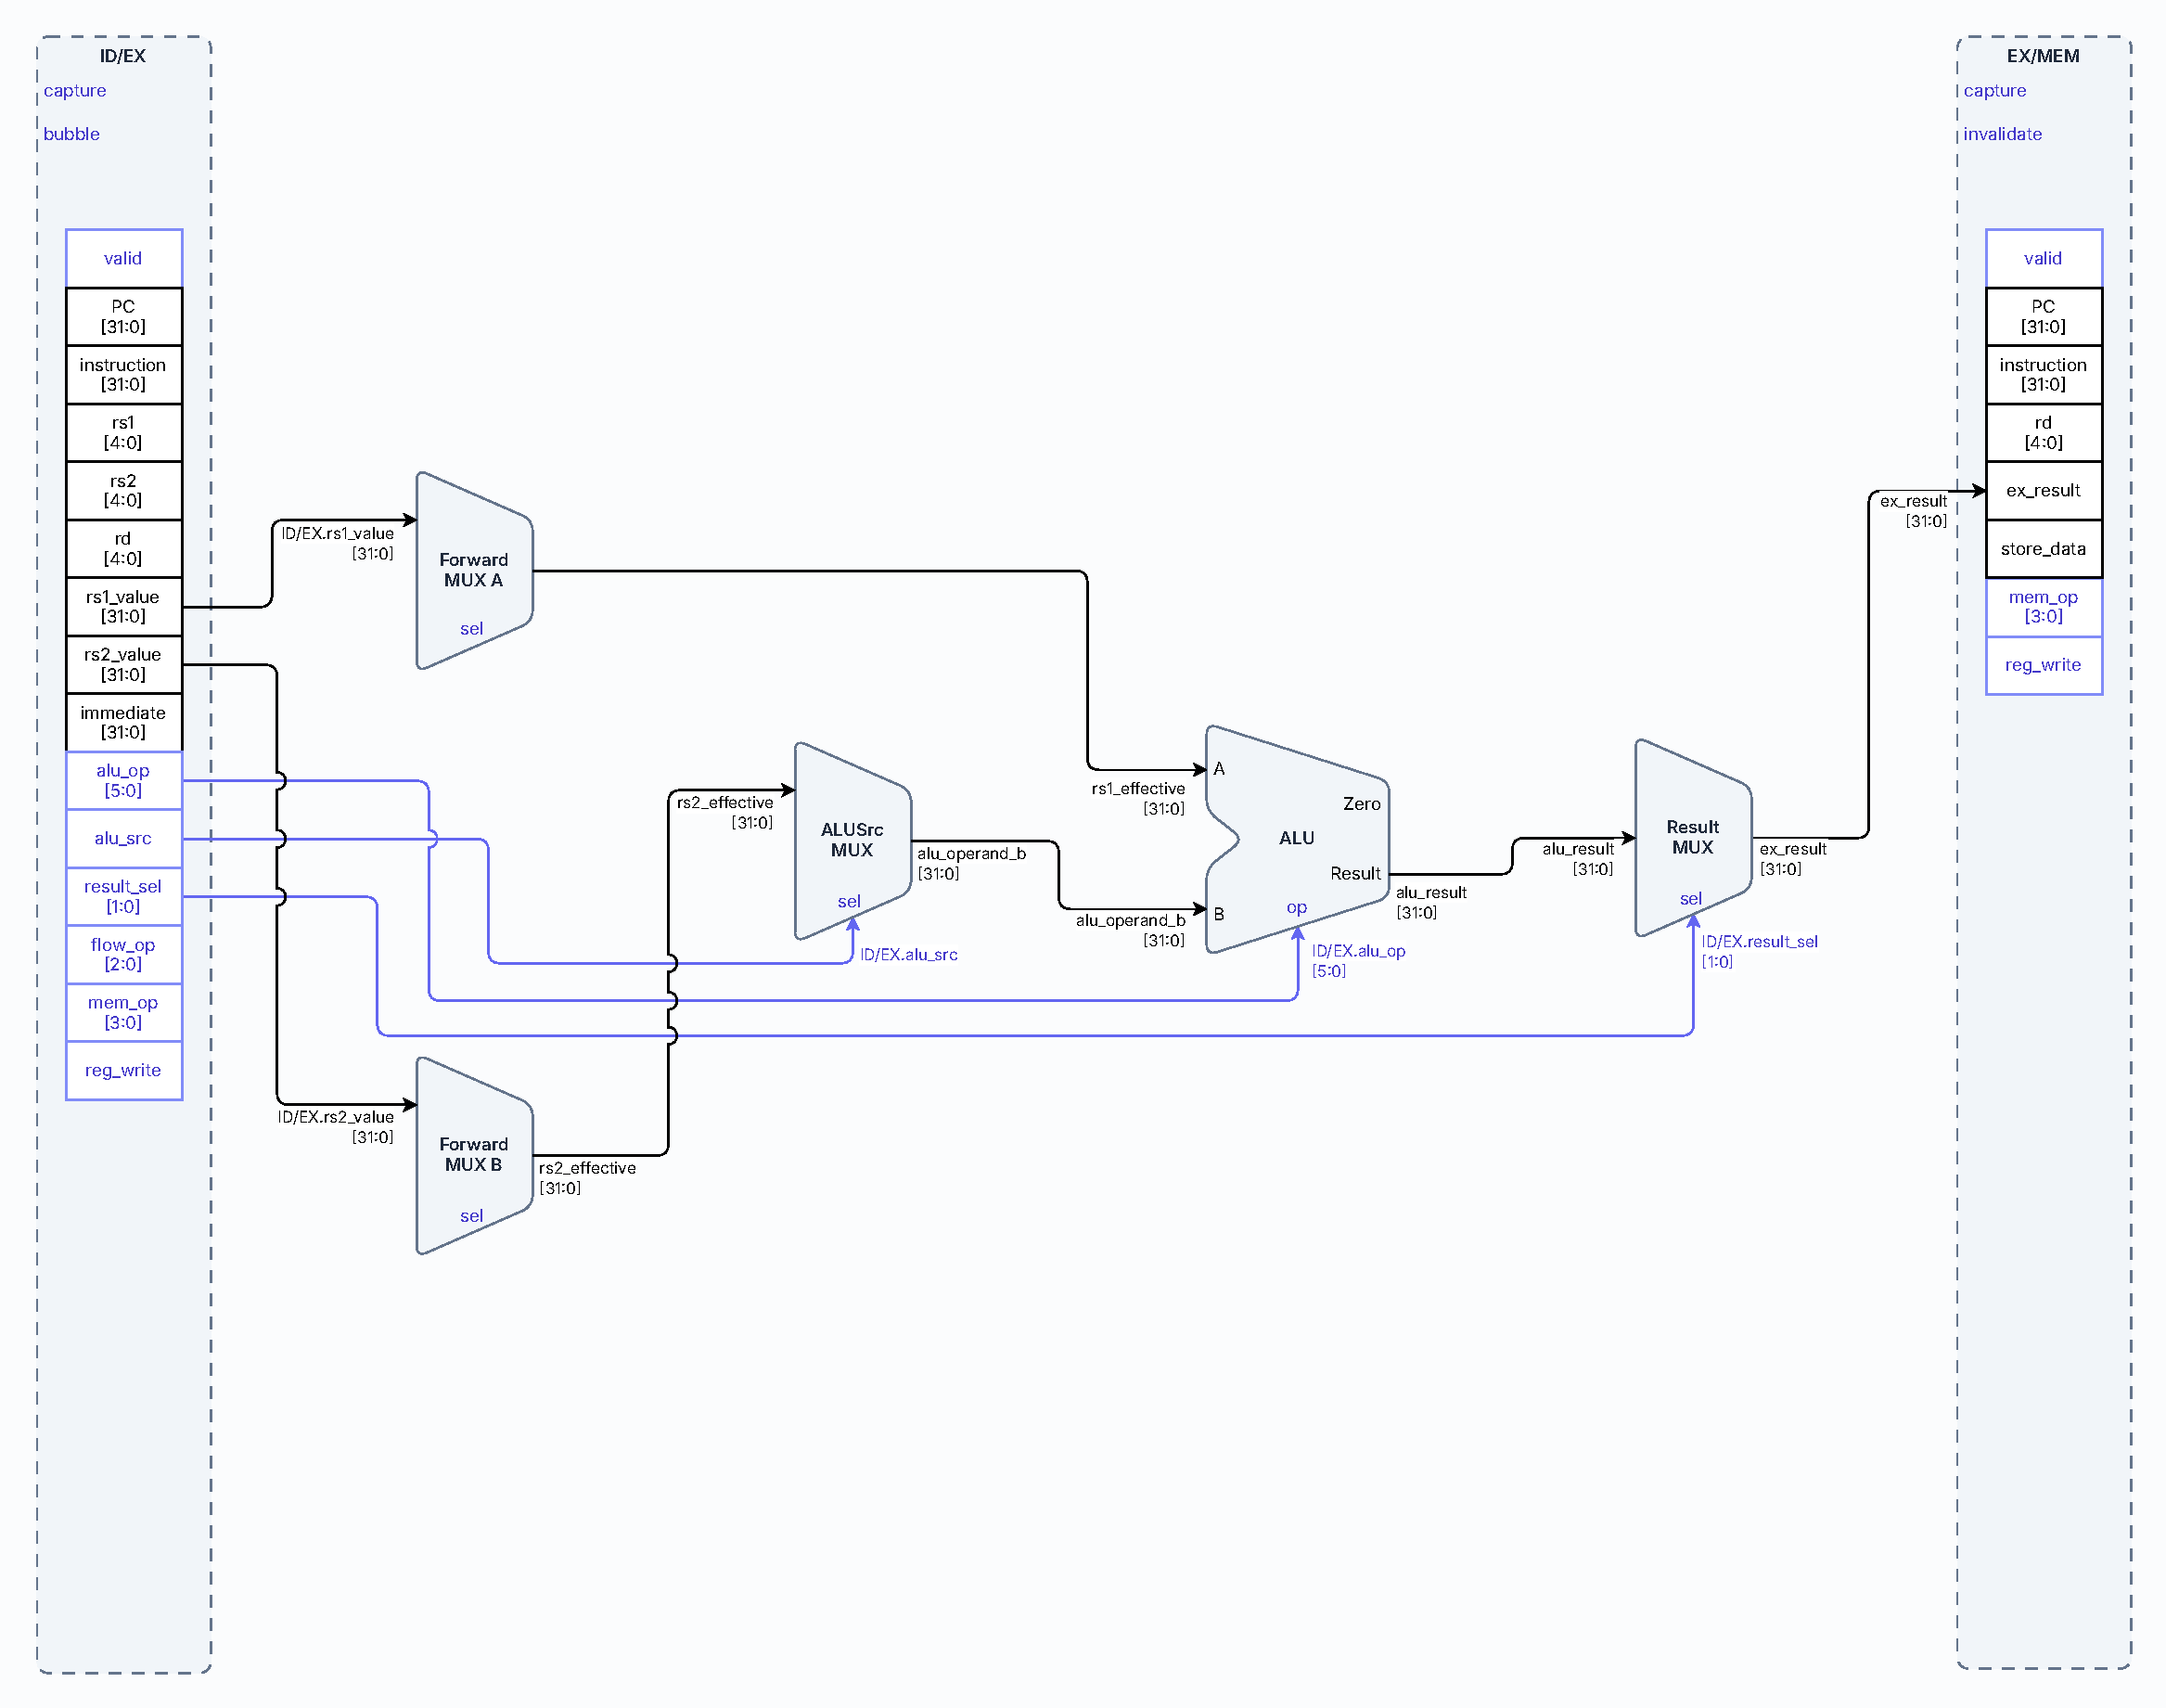
\includegraphics[width=0.92\textwidth]{ex-r.pdf}
  \caption{Recorrido de EX para una operación de registro: forwarding,
  ALU y selección del resultado.}
  \label{fig:etapa-ex}
\end{figure}

\subsection{Resultados y validaciones}

La ALU ejecuta la operación indicada por \code{alu_op}. Luego,
\code{result_sel} elige qué valor representa el resultado de la instrucción:
el resultado de la ALU, el inmediato o el enlace \code{PC + 4}. Para un load o
un store, ese resultado es la dirección efectiva; para \code{LUI} es el
inmediato y para \code{JAL}/\code{JALR} es el enlace. EX también valida la
alineación y el rango de los accesos a datos y de los destinos de control. Un
fault propio de EX tiene prioridad sobre el efecto normal de la misma
instrucción.

\begin{figure}[H]
  \centering
  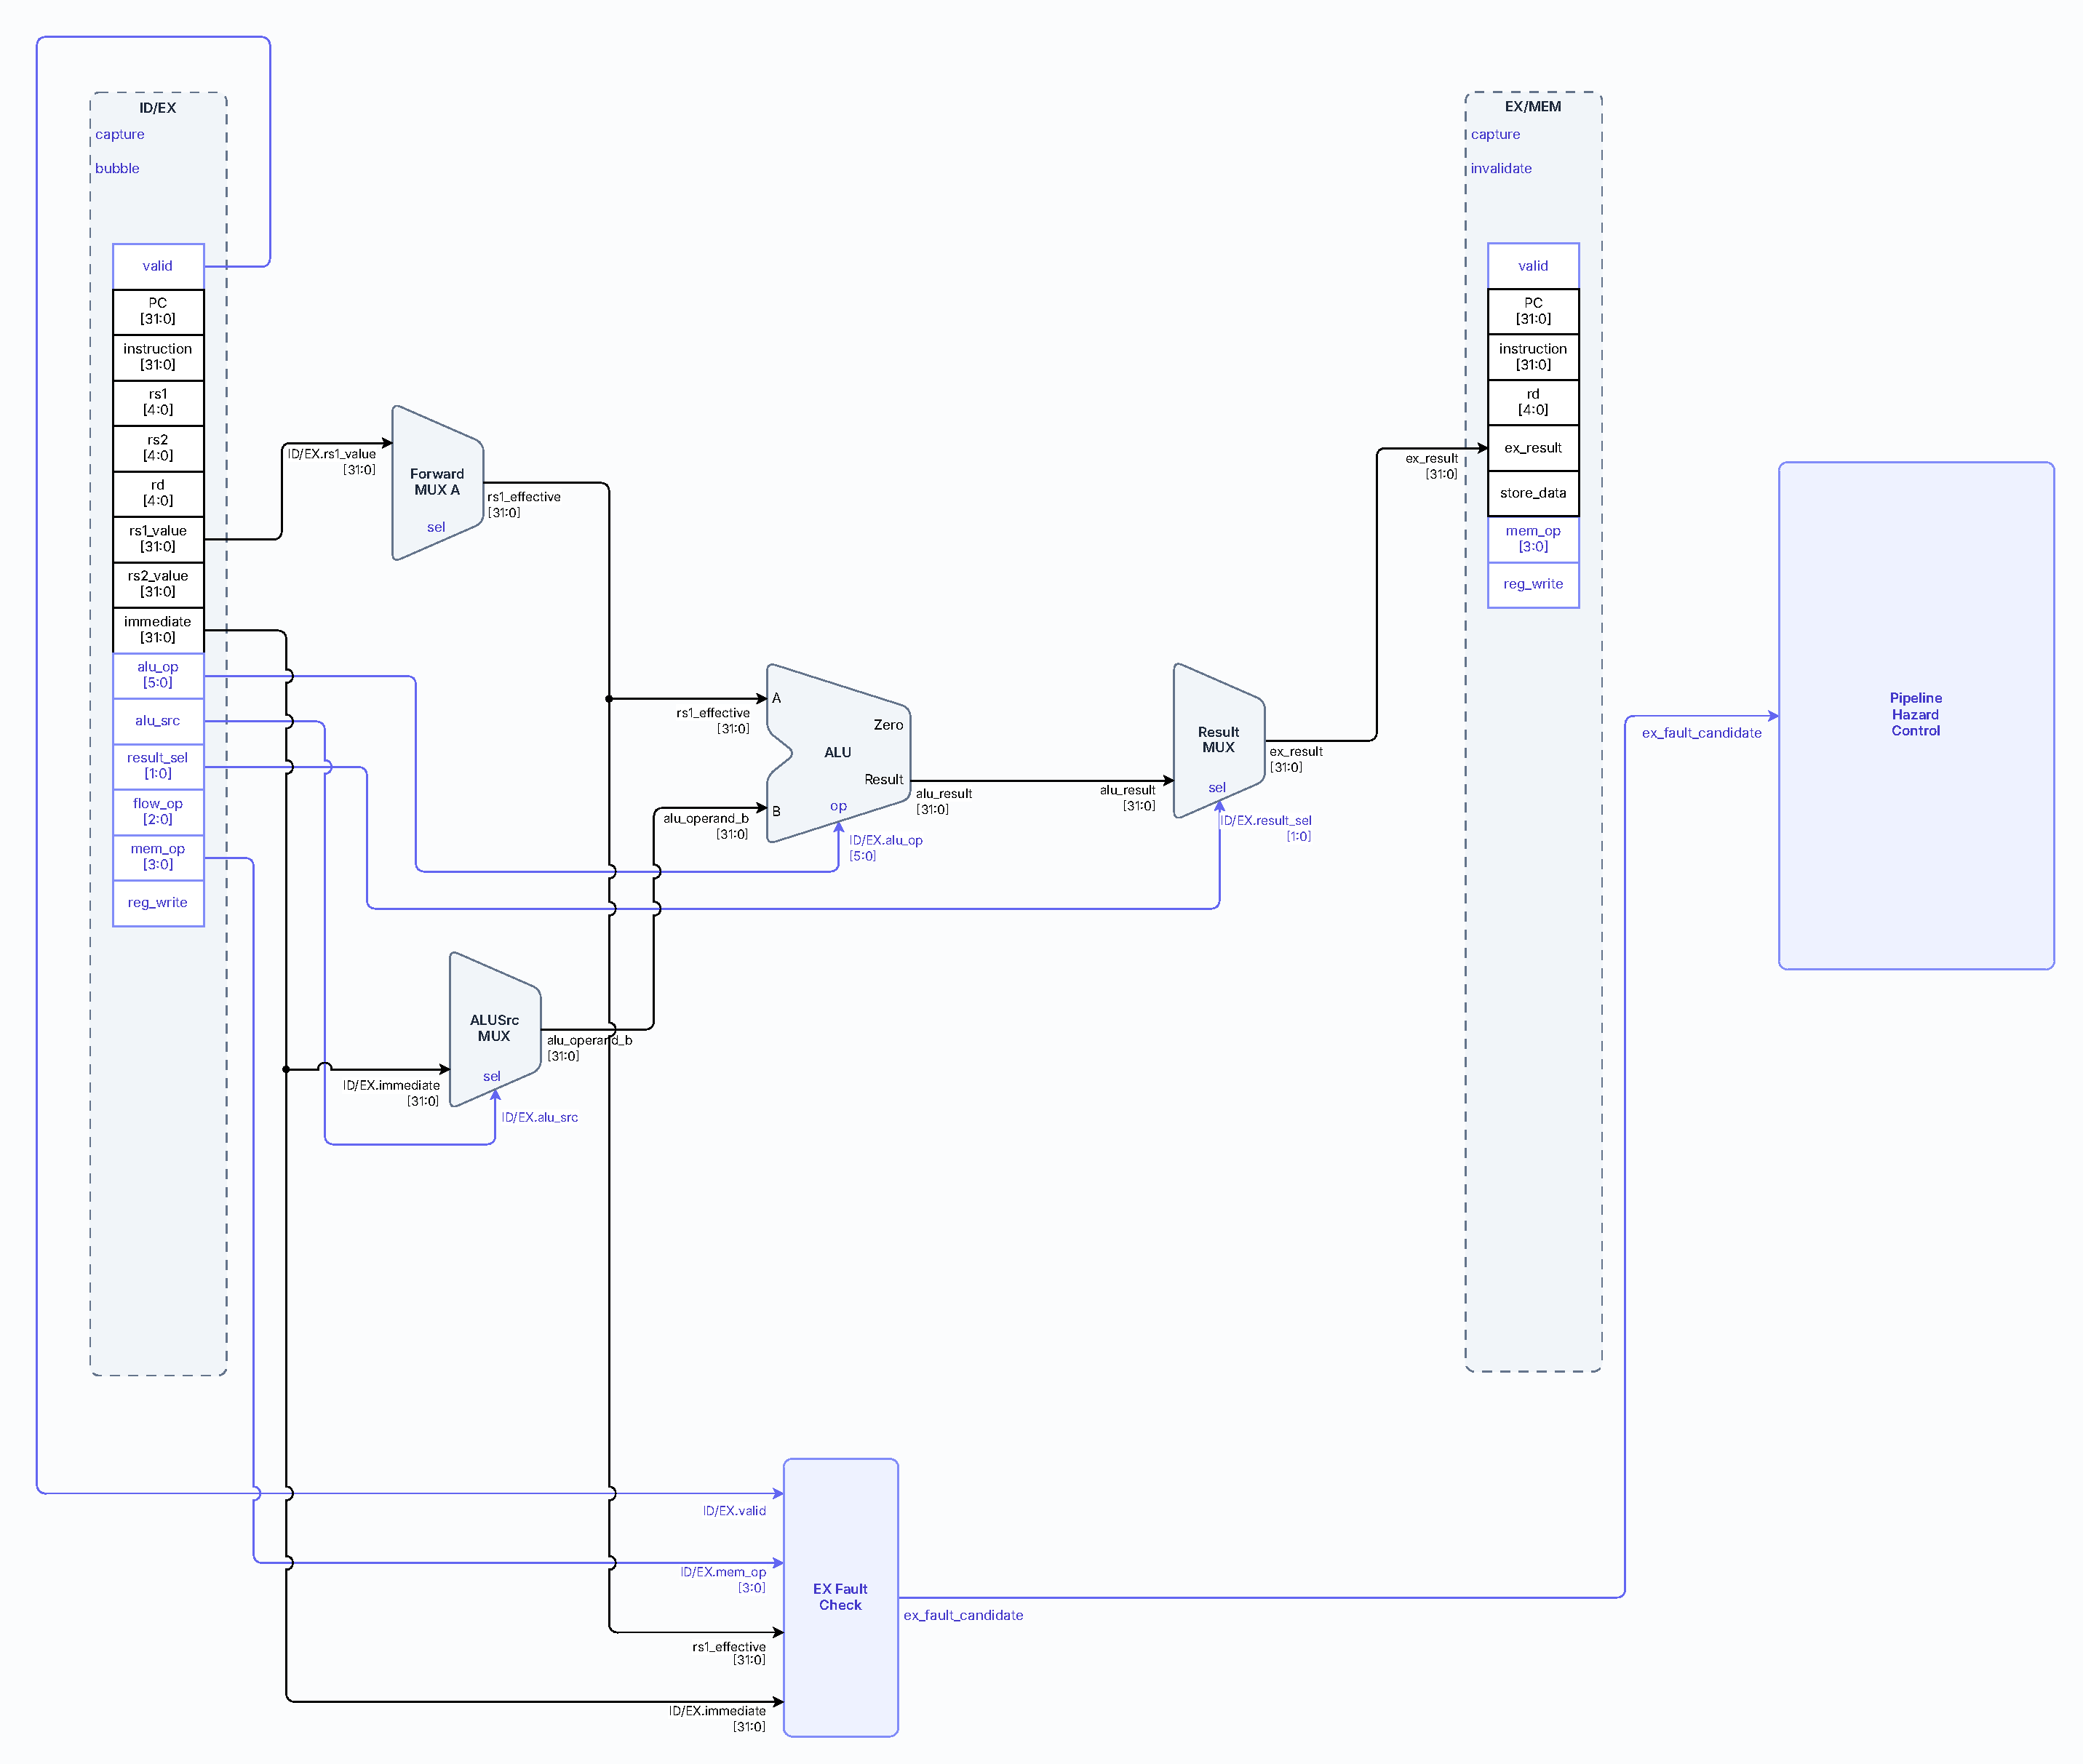
\includegraphics[width=0.80\textwidth]{ex-load.pdf}
  \caption{Recorrido de un load en EX: dirección efectiva, validación de
  alineación y rango, y preparación del acceso a MEM.}
  \label{fig:etapa-ex-load}
\end{figure}

\subsection{Cambios de flujo y terminación}

Los cambios de flujo se resuelven con los operandos efectivos:

\begin{itemize}
  \item \code{BEQ} toma el branch cuando ambos operandos son iguales y
    \code{BNE} cuando son distintos. Su destino, al igual que el de \code{JAL},
    es \code{ID/EX.pc + immediate}.
  \item \code{JALR} forma \code{(rs1_effective + immediate) \& 0xFFFFFFFE};
    después se comprueba que el destino esté alineado a cuatro bytes.
  \item \code{JAL} y \code{JALR} calculan además el enlace
    \code{ID/EX.pc + 4}, que se conserva para WB cuando no hay fault.
\end{itemize}

Cuando un branch tomado, \code{JAL} o \code{JALR} solicita un redirect, el
control actualiza el PC e invalida las instrucciones posteriores que ya habían
ingresado al pipeline. La instrucción de control sigue hacia \code{EX/MEM} para
conservar su enlace o completar su recorrido temporal. \code{halt}, en cambio,
se confirma en EX y no ingresa válidamente a \code{EX/MEM}; las instrucciones
anteriores todavía pueden completar durante el drenado.

\section{Memory (MEM)}

MEM recibe desde \code{EX/MEM} una instrucción cuya dirección efectiva ya fue
calculada y validada en EX. A partir de \code{mem_op}, determina si debe leer,
escribir o simplemente transportar el resultado de EX. La etapa es
combinacional entre \code{EX/MEM} y \code{MEM/WB}, salvo por la escritura
síncrona que realiza un store en el flanco del ciclo efectivo.

Sus bloques principales son:

\begin{itemize}
  \item \textbf{\code{MEM Decode}:} interpreta \code{mem_op} y determina si
    hay un load, un store, el tamaño del acceso y si el load es unsigned.
  \item \textbf{\code{Data Memory}:} lee los bytes solicitados por un load o
    escribe los bytes habilitados por un store.
  \item \textbf{\code{Load Select / Extend}:} selecciona el byte, halfword o
    word correspondiente al offset y lo extiende a 32 bits.
  \item \textbf{\code{DMEM Write Control}:} genera \code{dmem_store_fire} y la
    máscara de bytes que utiliza un store.
  \item \textbf{\code{WB Value MUX}:} elige entre el dato cargado y el
    resultado que ya venía de EX.
  \item \textbf{\code{MEM/WB Update Control} y registro \code{MEM/WB}:}
    capturan el valor final y los controles que necesita WB.
\end{itemize}

La figura~\ref{fig:etapa-mem} muestra la organización completa de la etapa.

\begin{figure}[H]
  \centering
  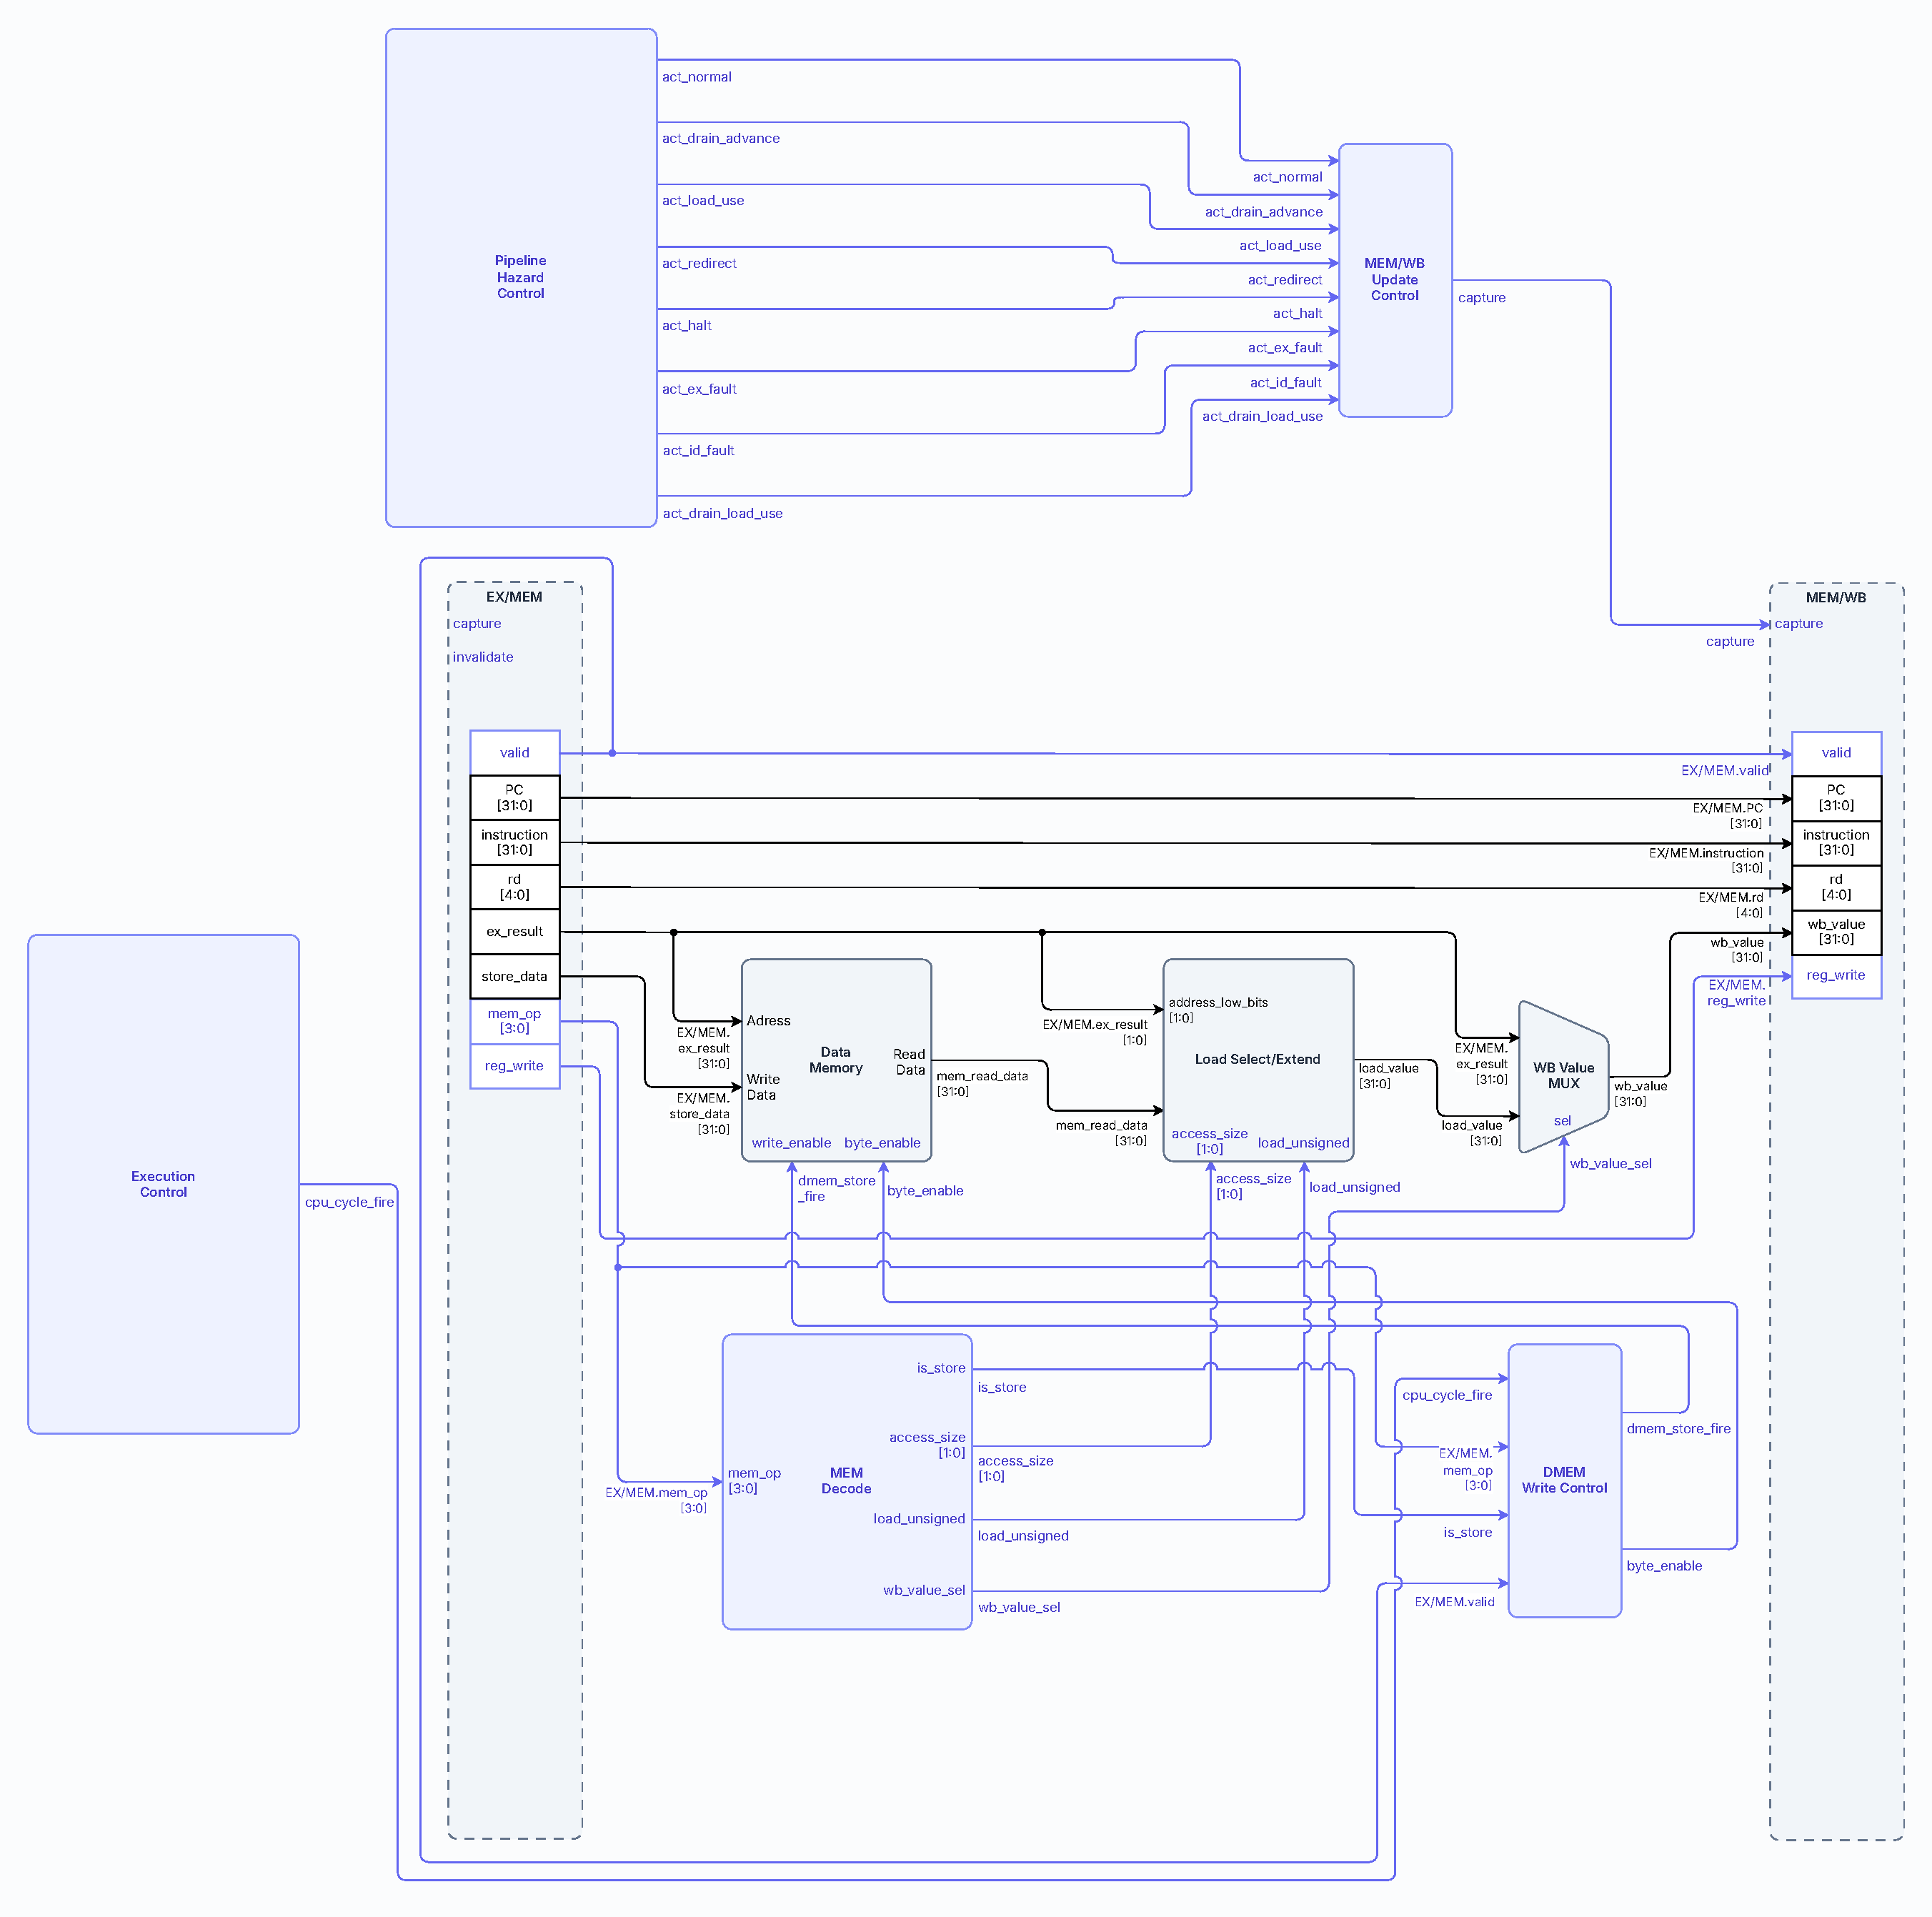
\includegraphics[width=0.80\textwidth]{mem-organizacion.pdf}
  \caption{Organización de MEM: acceso a DMEM, selección y extensión de loads,
  máscara de stores y selección del valor de writeback.}
  \label{fig:etapa-mem}
\end{figure}

\subsection{Loads y selección del dato}

Para un load, \code{EX/MEM.ex_result} es la dirección efectiva. \code{Data
Memory} entrega la palabra alineada de cuatro bytes y \code{Load Select / Extend}
utiliza el offset y el tamaño del acceso para seleccionar el byte, halfword o
word solicitado. Luego aplica extensión con signo o sin signo según
\code{mem_op}. El resultado de 32 bits queda listo para el camino de
writeback.

\subsection{Stores y escritura de DMEM}

Para un store, \code{EX/MEM.ex_result} aporta la dirección y
\code{EX/MEM.store_data} aporta el dato. \code{DMEM Write Control} solo activa
la escritura cuando se cumplen simultáneamente estas condiciones:

\begin{itemize}
  \item el ciclo de CPU es efectivo;
  \item \code{EX/MEM} contiene una entrada válida;
  \item \code{mem_op} identifica un store.
\end{itemize}

La máscara depende del tamaño: un byte para \code{SB}, dos para \code{SH} y
cuatro para \code{SW}. La memoria desplaza esa máscara según los bits bajos de
la dirección y actualiza tanto los datos como sus marcas de validez. Un store
anterior puede completar su efecto en el mismo ciclo en que se confirma el
fault o \code{halt} de una instrucción posterior.

\subsection{Selección del valor de writeback}

La selección de resultados se reparte entre EX y MEM. EX ya eligió entre el
resultado de la ALU, el inmediato y el enlace \code{PC + 4}, y guardó ese valor
en \code{EX/MEM.ex_result}. En MEM, \code{WB Value MUX} selecciona entre ese
resultado y el dato producido por un load. El valor único elegido se captura en
\code{MEM/WB.wb_value}; WB no vuelve a seleccionar su origen.

La estructura detallada de estos caminos se encuentra en
\doc{architecture/cpu/stage_mem.md}{la etapa MEM}.

\section{Write Back (WB)}

WB es la última etapa del recorrido. Recibe desde \code{MEM/WB} el resultado
final de la instrucción y decide si debe hacerlo visible en el banco de
registros. No vuelve a calcular ni a seleccionar el origen del dato: esa
selección ya ocurrió en MEM.

Sus bloques y conexiones principales son:

\begin{itemize}
  \item \textbf{\code{WB Bypass Control}:} forma la condición efectiva de
    escritura y los controles de bypass hacia ID.
  \item \textbf{Puerto de escritura del \code{Register File}:} recibe
    \code{MEM/WB.rd}, \code{MEM/WB.wb_value} y la habilitación de WB.
  \item \textbf{\code{RS1 Bypass MUX} y \code{RS2 Bypass MUX}:} pueden entregar
    a ID el mismo valor de \code{MEM/WB.wb_value} cuando hay una lectura
    coincidente.
  \item \textbf{Registro \code{MEM/WB}:} conserva el resultado final y la
    identidad de la instrucción que WB observa y utiliza.
\end{itemize}

La figura~\ref{fig:etapa-wb} muestra la organización de la etapa.

\begin{figure}[H]
  \centering
  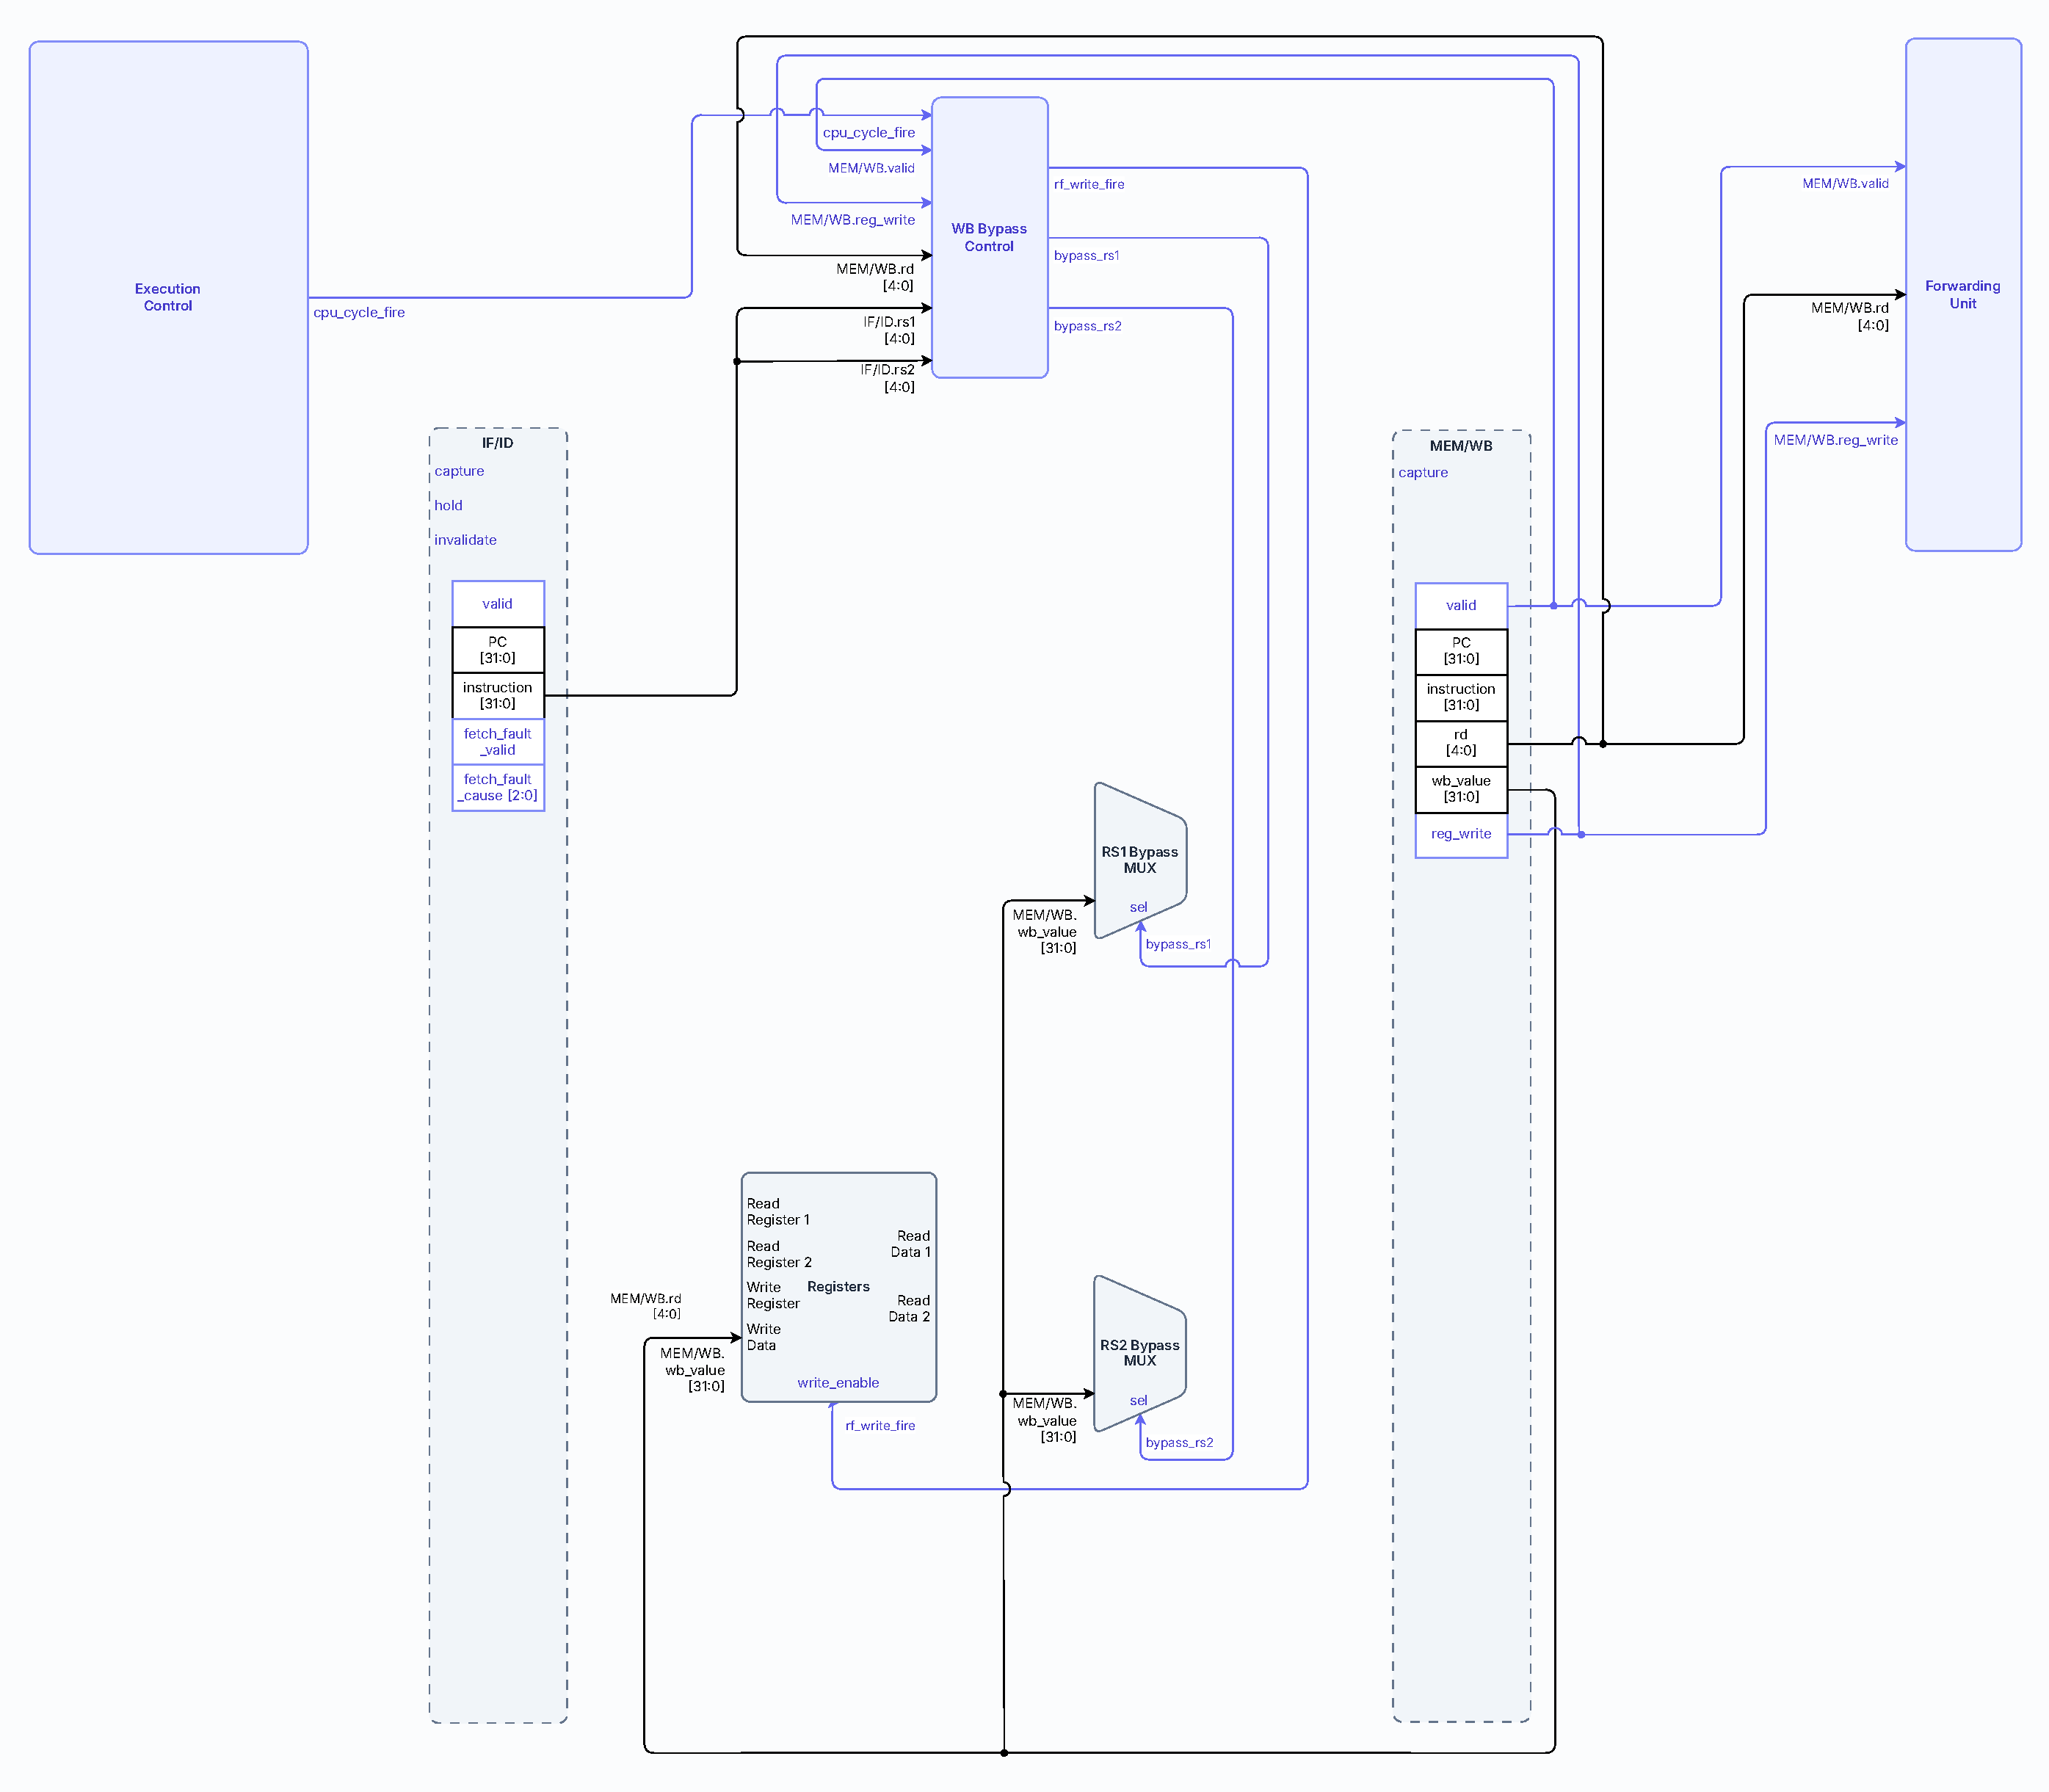
\includegraphics[width=0.92\textwidth]{wb-organizacion.pdf}
  \caption{Organización de WB: escritura del banco de registros y generación
  de los controles de bypass hacia ID.}
  \label{fig:etapa-wb}
\end{figure}

\subsection{Escritura efectiva}

La escritura se realiza de forma síncrona y solo ocurre cuando se cumplen
simultáneamente estas condiciones:

\begin{itemize}
  \item el ciclo de CPU es efectivo;
  \item \code{MEM/WB} contiene una entrada válida;
  \item \code{reg_write} está activo;
  \item el destino es distinto de \code{x0}.
\end{itemize}

Cuando todas se cumplen, WB ejecuta conceptualmente:

\begin{codebox}
RF[MEM/WB.rd] <- MEM/WB.wb_value
\end{codebox}

Una entrada inválida no produce efectos aunque sus campos conserven valores
residuales. Stores y branches pueden atravesar WB con \code{reg_write=0}; en
ese caso solo conservan su identidad para la observación del pipeline.

\subsection{Bypass y forwarding}

La misma escritura efectiva habilita el bypass \tech{WB}$\rightarrow$\tech{ID}.
Si ID lee el registro que WB está escribiendo, el mux correspondiente entrega
directamente \code{MEM/WB.wb_value} en lugar del valor anterior del banco. De
esta forma, el resultado nuevo está disponible en ID durante el mismo ciclo y
la arquitectura no depende de que el almacenamiento sea write-first o
read-first.

Ese mismo \code{MEM/WB.wb_value} también queda disponible para el forwarding
desde MEM/WB hacia EX. WB no crea un valor adicional: reutiliza el resultado
final que MEM ya consolidó, ya provenga de la ALU, de \code{LUI}, del enlace de
un salto o de un load. La condición exacta se detalla en
\doc{architecture/cpu/stage_wb.md}{Etapa WB}.

\section{Registros interetapa y validez}\label{sec:registros-interetapa}

\subsection{Avance y captura}

Los cuatro registros interetapa son \code{if_id_register},
\code{id_ex_register}, \code{ex_mem_register} y \code{mem_wb_register}.
Cada uno captura el trabajo producido por la etapa anterior en el flanco
habilitado. La actualización se basa en los valores previos al flanco; una
instrucción avanza como máximo una etapa por ciclo.

\subsection{Validez y estados del pipeline}

La validez es parte del contrato del pipeline, no un detalle de
implementación. Un registro puede conservar bits residuales en sus otros
campos, pero solo una entrada válida representa una instrucción activa y puede
producir efectos. Esta distinción permite:

\begin{itemize}
  \item representar una burbuja sin ejecutar una instrucción inexistente;
  \item retener una instrucción durante un stall sin invalidarla;
  \item descartar instrucciones de un camino abandonado sin borrar todos sus
    campos;
  \item distinguir un candidato de fault de una instrucción activa.
\end{itemize}

Una entrada inválida no participa en forwarding, bypass ni writeback. En el
caso particular de \code{IF/ID}, \code{valid=0} y
\code{fetch_fault_valid=1} representan un candidato de fault de fetch, no una
instrucción ejecutable. La selección exacta entre captura, retención, burbuja e
invalidación depende de la acción elegida por el control del pipeline.

\subsection{Campos transportados y observables}

Los 34 campos funcionales de los latches suman 504 bits y se observan en Debug.
La tabla~\ref{tab:campos-latches} detalla los campos que transporta cada
registro y el ancho de cada conjunto.

\begin{table}[H]
  \centering
  \footnotesize
  \setlength{\tabcolsep}{3pt}
  \begin{tabularx}{\textwidth}{L{1.7cm}Y r}
    \toprule
    \textbf{Registro} & \textbf{Campos (ancho en bits)} & \textbf{Total} \\
    \midrule
    \code{IF/ID} & \code{valid(1)}, \code{pc(32)}, \code{instruction(32)},
    \code{fetch_fault_valid(1)}, \code{fetch_fault_cause(3)} & 69 \\
    \addlinespace
    \code{ID/EX} & \code{valid(1)}, \code{pc(32)}, \code{instruction(32)},
    \code{rs1(5)}, \code{rs2(5)}, \code{rd(5)}, \code{rs1_value(32)},
    \code{rs2_value(32)}, \code{immediate(32)}, \code{alu_op(6)},
    \code{alu_src(1)}, \code{result_sel(2)}, \code{flow_op(3)},
    \code{mem_op(4)}, \code{reg_write(1)} & 193 \\
    \addlinespace
    \code{EX/MEM} & \code{valid(1)}, \code{pc(32)}, \code{instruction(32)},
    \code{rd(5)}, \code{reg_write(1)}, \code{mem_op(4)}, \code{ex_result(32)},
    \code{store_data(32)} & 139 \\
    \addlinespace
    \code{MEM/WB} & \code{valid(1)}, \code{pc(32)}, \code{instruction(32)},
    \code{rd(5)}, \code{reg_write(1)}, \code{wb_value(32)} & 103 \\
    \bottomrule
  \end{tabularx}
  \caption{Campos funcionales de los registros interetapa.}
  \label{tab:campos-latches}
\end{table}

Estos campos conservan la identidad de la instrucción, los datos que necesita
la etapa siguiente y las señales de control que deben atravesar el pipeline.
La validez determina cuándo ese contenido tiene significado arquitectónico y
también permite que Debug distinga trabajo activo de datos residuales.

\section{Branches, jumps, \code{halt} y faults}

\subsection{Branches, jumps y redirects}

Los branches y jumps se resuelven en EX. \code{Flow Control} compara los
operandos cuando corresponde y produce la solicitud de redirect junto con el
destino calculado. \code{Pipeline Hazard Control} arbitra esa solicitud frente
a los faults, \code{halt} y hazards que puedan aparecer en el mismo ciclo.

Cuando el redirect se confirma, el PC adopta el nuevo destino y se invalidan
las instrucciones más jóvenes que todavía estaban en IF o ID. La instrucción
que originó el cambio de flujo continúa hacia \code{EX/MEM}; así, \code{JAL} y
\code{JALR} pueden conservar su enlace para escribirlo posteriormente.
La figura~\ref{fig:etapa-branch} muestra este recorrido.

\begin{figure}[H]
  \centering
  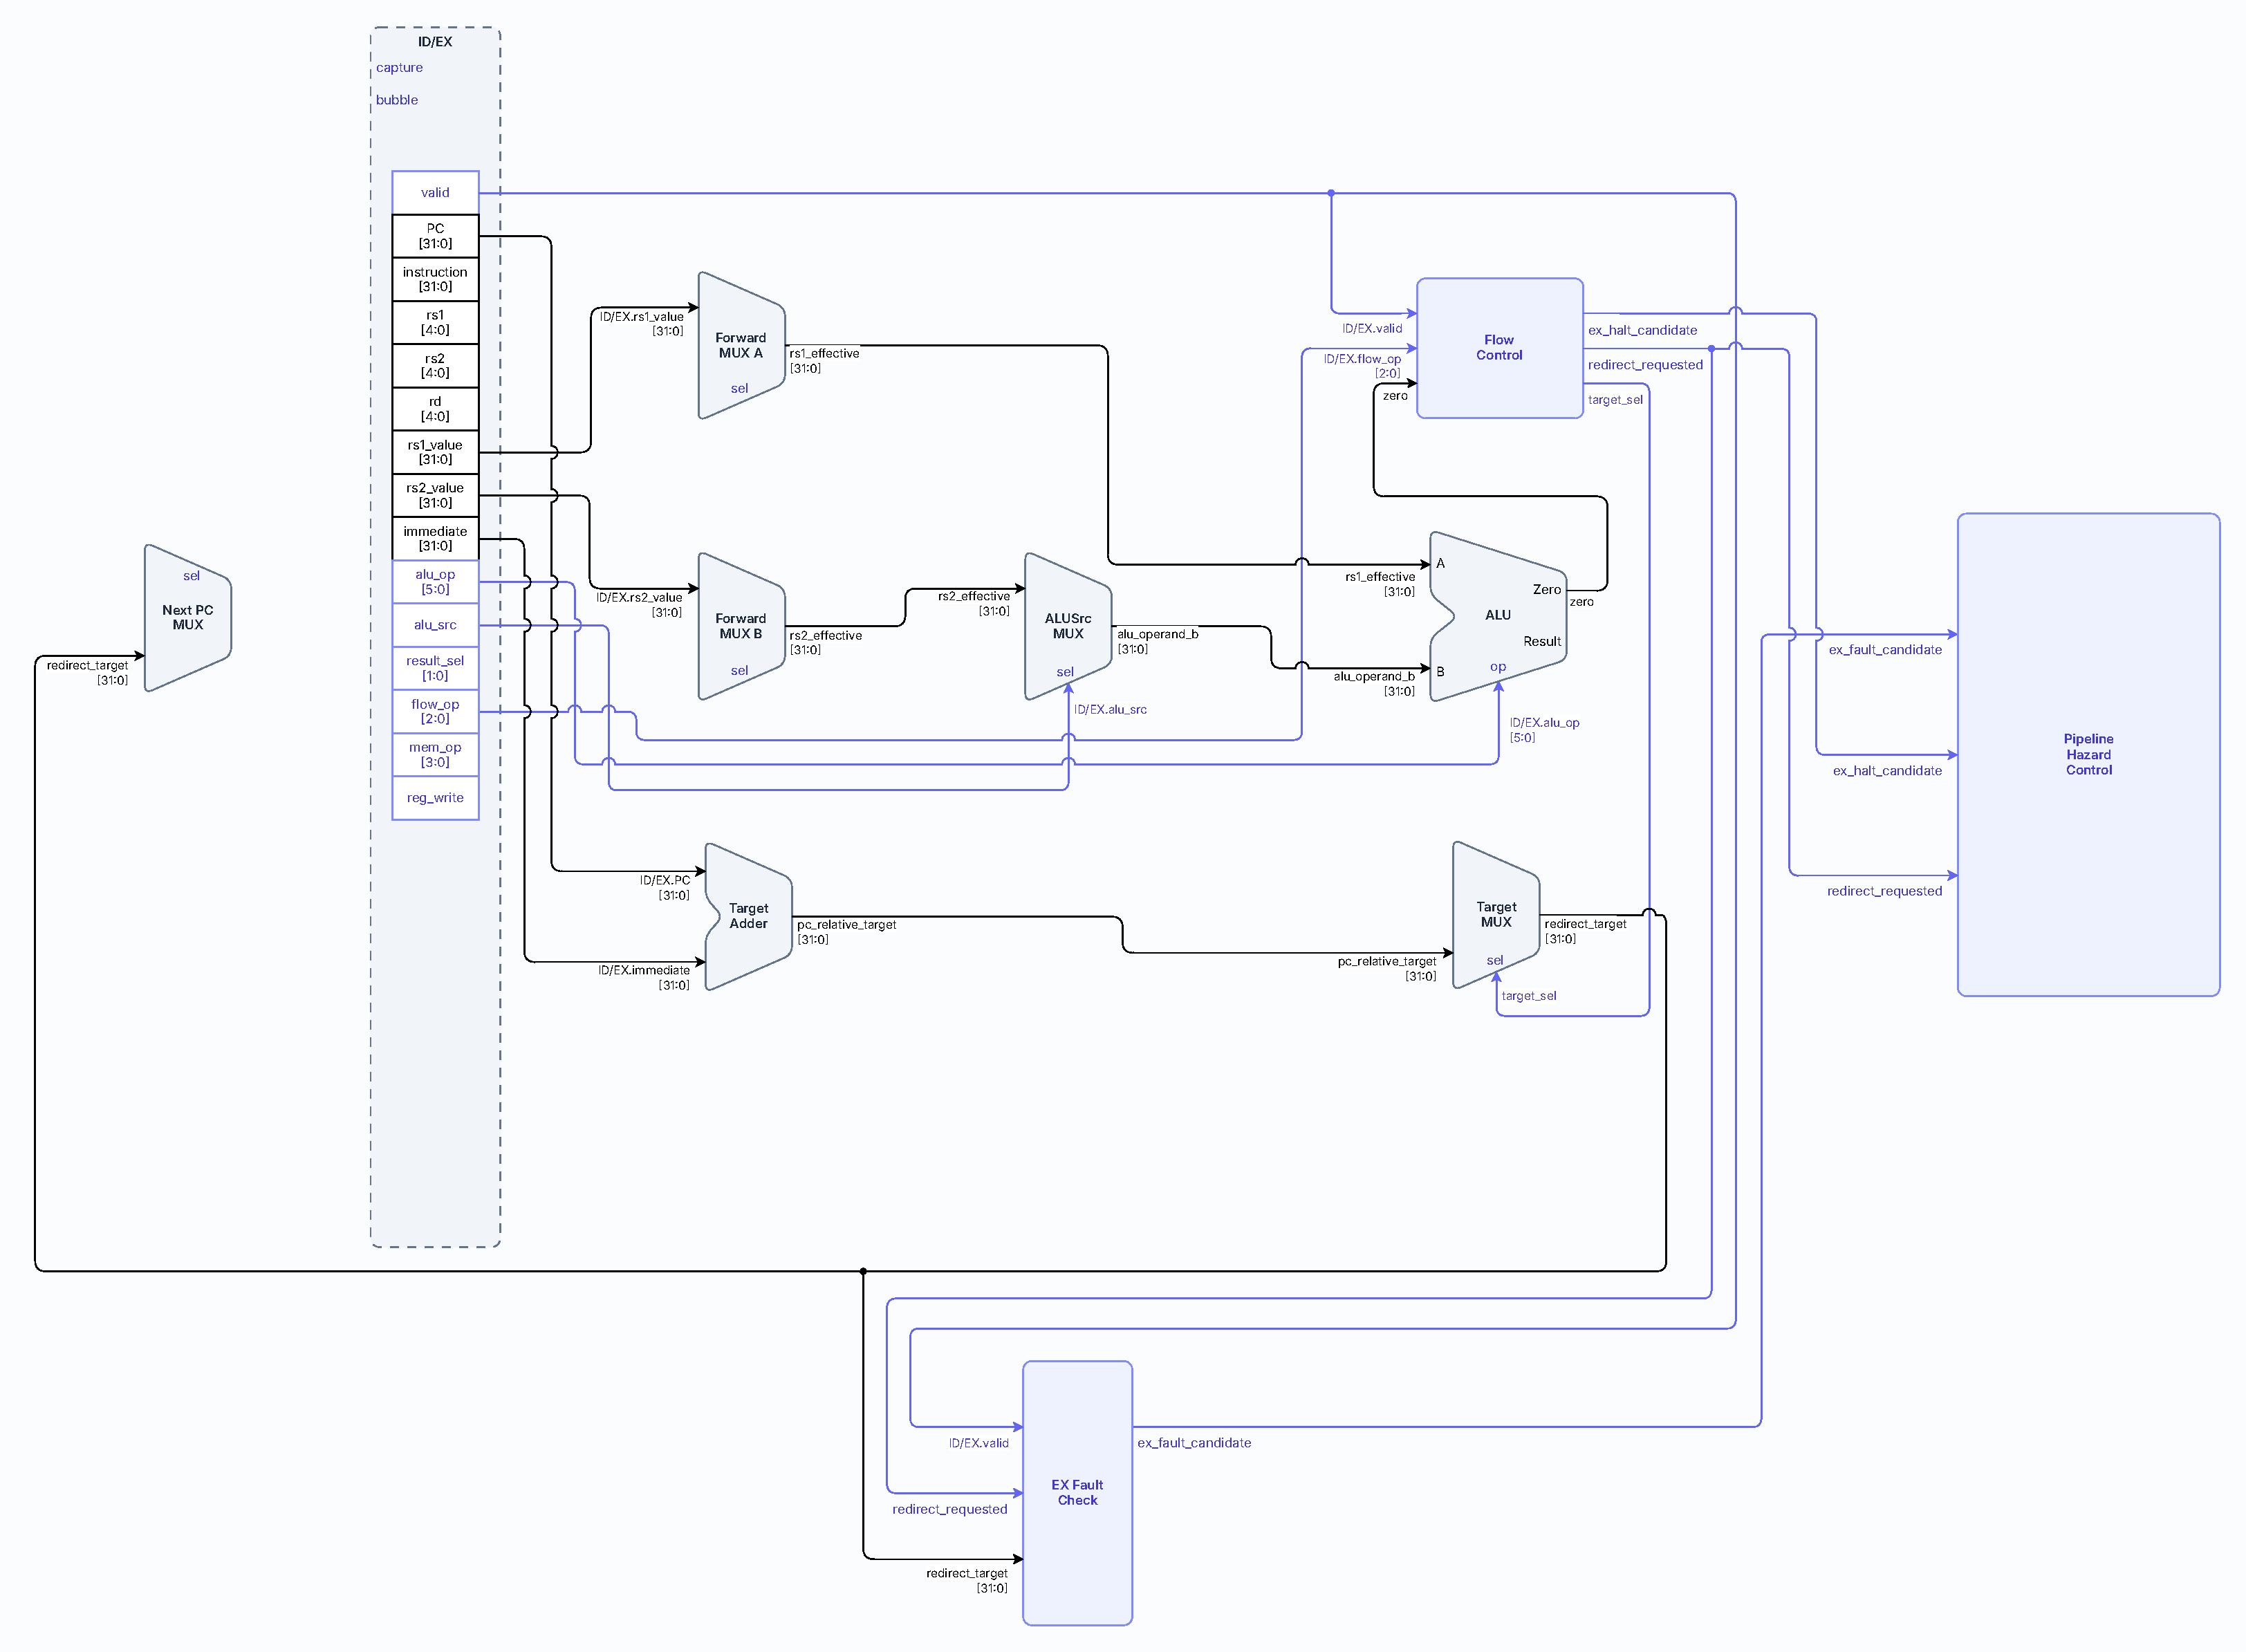
\includegraphics[width=0.92\textwidth]{ex-branch.pdf}
  \caption{Recorrido de un branch en EX: comparación, cálculo del destino y
  selección del próximo PC.}
  \label{fig:etapa-branch}
\end{figure}

\subsection{Origen y transporte de faults}

Un fault puede detectarse en tres puntos del pipeline:

\begin{itemize}
  \item \textbf{IF:} una búsqueda desalineada o fuera de la capacidad o de la
    imagen confirmada produce un candidato de fault de fetch.
  \item \textbf{ID:} una instrucción ilegal o un candidato de fetch transportado
    por \code{IF/ID} produce un candidato de fault de ID.
  \item \textbf{EX:} se detecta una dirección desalineada o fuera de rango en
    un acceso a DMEM, o un destino de control inválido.
\end{itemize}

La detección solo produce un candidato. La confirmación ocurre en un ciclo
efectivo, después de que \code{Pipeline Hazard Control} comprueba que ninguna
instrucción anterior produjo un evento con mayor prioridad. La figura
~\ref{fig:fetch-fault} muestra cómo un candidato de IF se transporta por
\code{IF/ID} antes de confirmarse en ID.

\subsection{Prioridad y precisión}

La confirmación respeta el orden del programa. La prioridad entre eventos es:

\begin{enumerate}
  \item fault propio de EX;
  \item \code{halt} en EX;
  \item redirect en EX;
  \item fault en ID;
  \item dependencia \code{load-use};
  \item avance normal.
\end{enumerate}

Cuando se confirma un fault, la instrucción causante y las posteriores se
descartan, mientras que las anteriores conservan sus efectos válidos. La causa
y el PC de la instrucción que falló se capturan una sola vez por sesión y se
conservan hasta el estado terminal. El diseño no necesita rollback: la
precisión se obtiene controlando qué instrucciones pueden producir efectos.

Las causas se codifican con tres bits. El código \code{011} queda reservado y
no representa una causa válida:

\begin{center}
  \begin{tabular}{clp{8.5cm}}
    \toprule
    \textbf{Código} & \textbf{Causa} & \textbf{Descripción} \\
    \midrule
    \code{000} & Instrucción desalineada & El PC no es múltiplo de cuatro. \\
    \code{001} & Falla de acceso a instrucción & La búsqueda de cuatro bytes queda fuera de la capacidad de IMEM o de la imagen confirmada. \\
    \code{010} & Instrucción ilegal & La palabra obtenida no coincide con ninguna codificación implementada. \\
    \code{011} & Reservado & No corresponde a una causa válida. \\
    \code{100} & Load desalineado & La dirección no cumple la alineación requerida por el tamaño del load. \\
    \code{101} & Falla de acceso a load & Alguno de los bytes solicitados por el load queda fuera del rango de DMEM. Una dirección dentro de DMEM que nunca fue escrita no produce este fault: el load obtiene cero lógico. \\
    \code{110} & Store desalineado & La dirección no cumple la alineación requerida por el tamaño del store. \\
    \code{111} & Falla de acceso a store & Alguno de los bytes que escribiría el store queda fuera del rango de DMEM. \\
    \bottomrule
  \end{tabular}
\end{center}

\subsection{\code{halt} y drenado}

\code{halt} se confirma en EX y no ingresa válidamente a \code{EX/MEM}. Las
instrucciones más jóvenes se invalidan, mientras que las anteriores que ya
están en MEM o WB continúan y pueden completar sus efectos. El sistema entra
en drenado y alcanza el estado terminal cuando el pipeline queda vacío.

\begin{figure}[H]
  \centering
  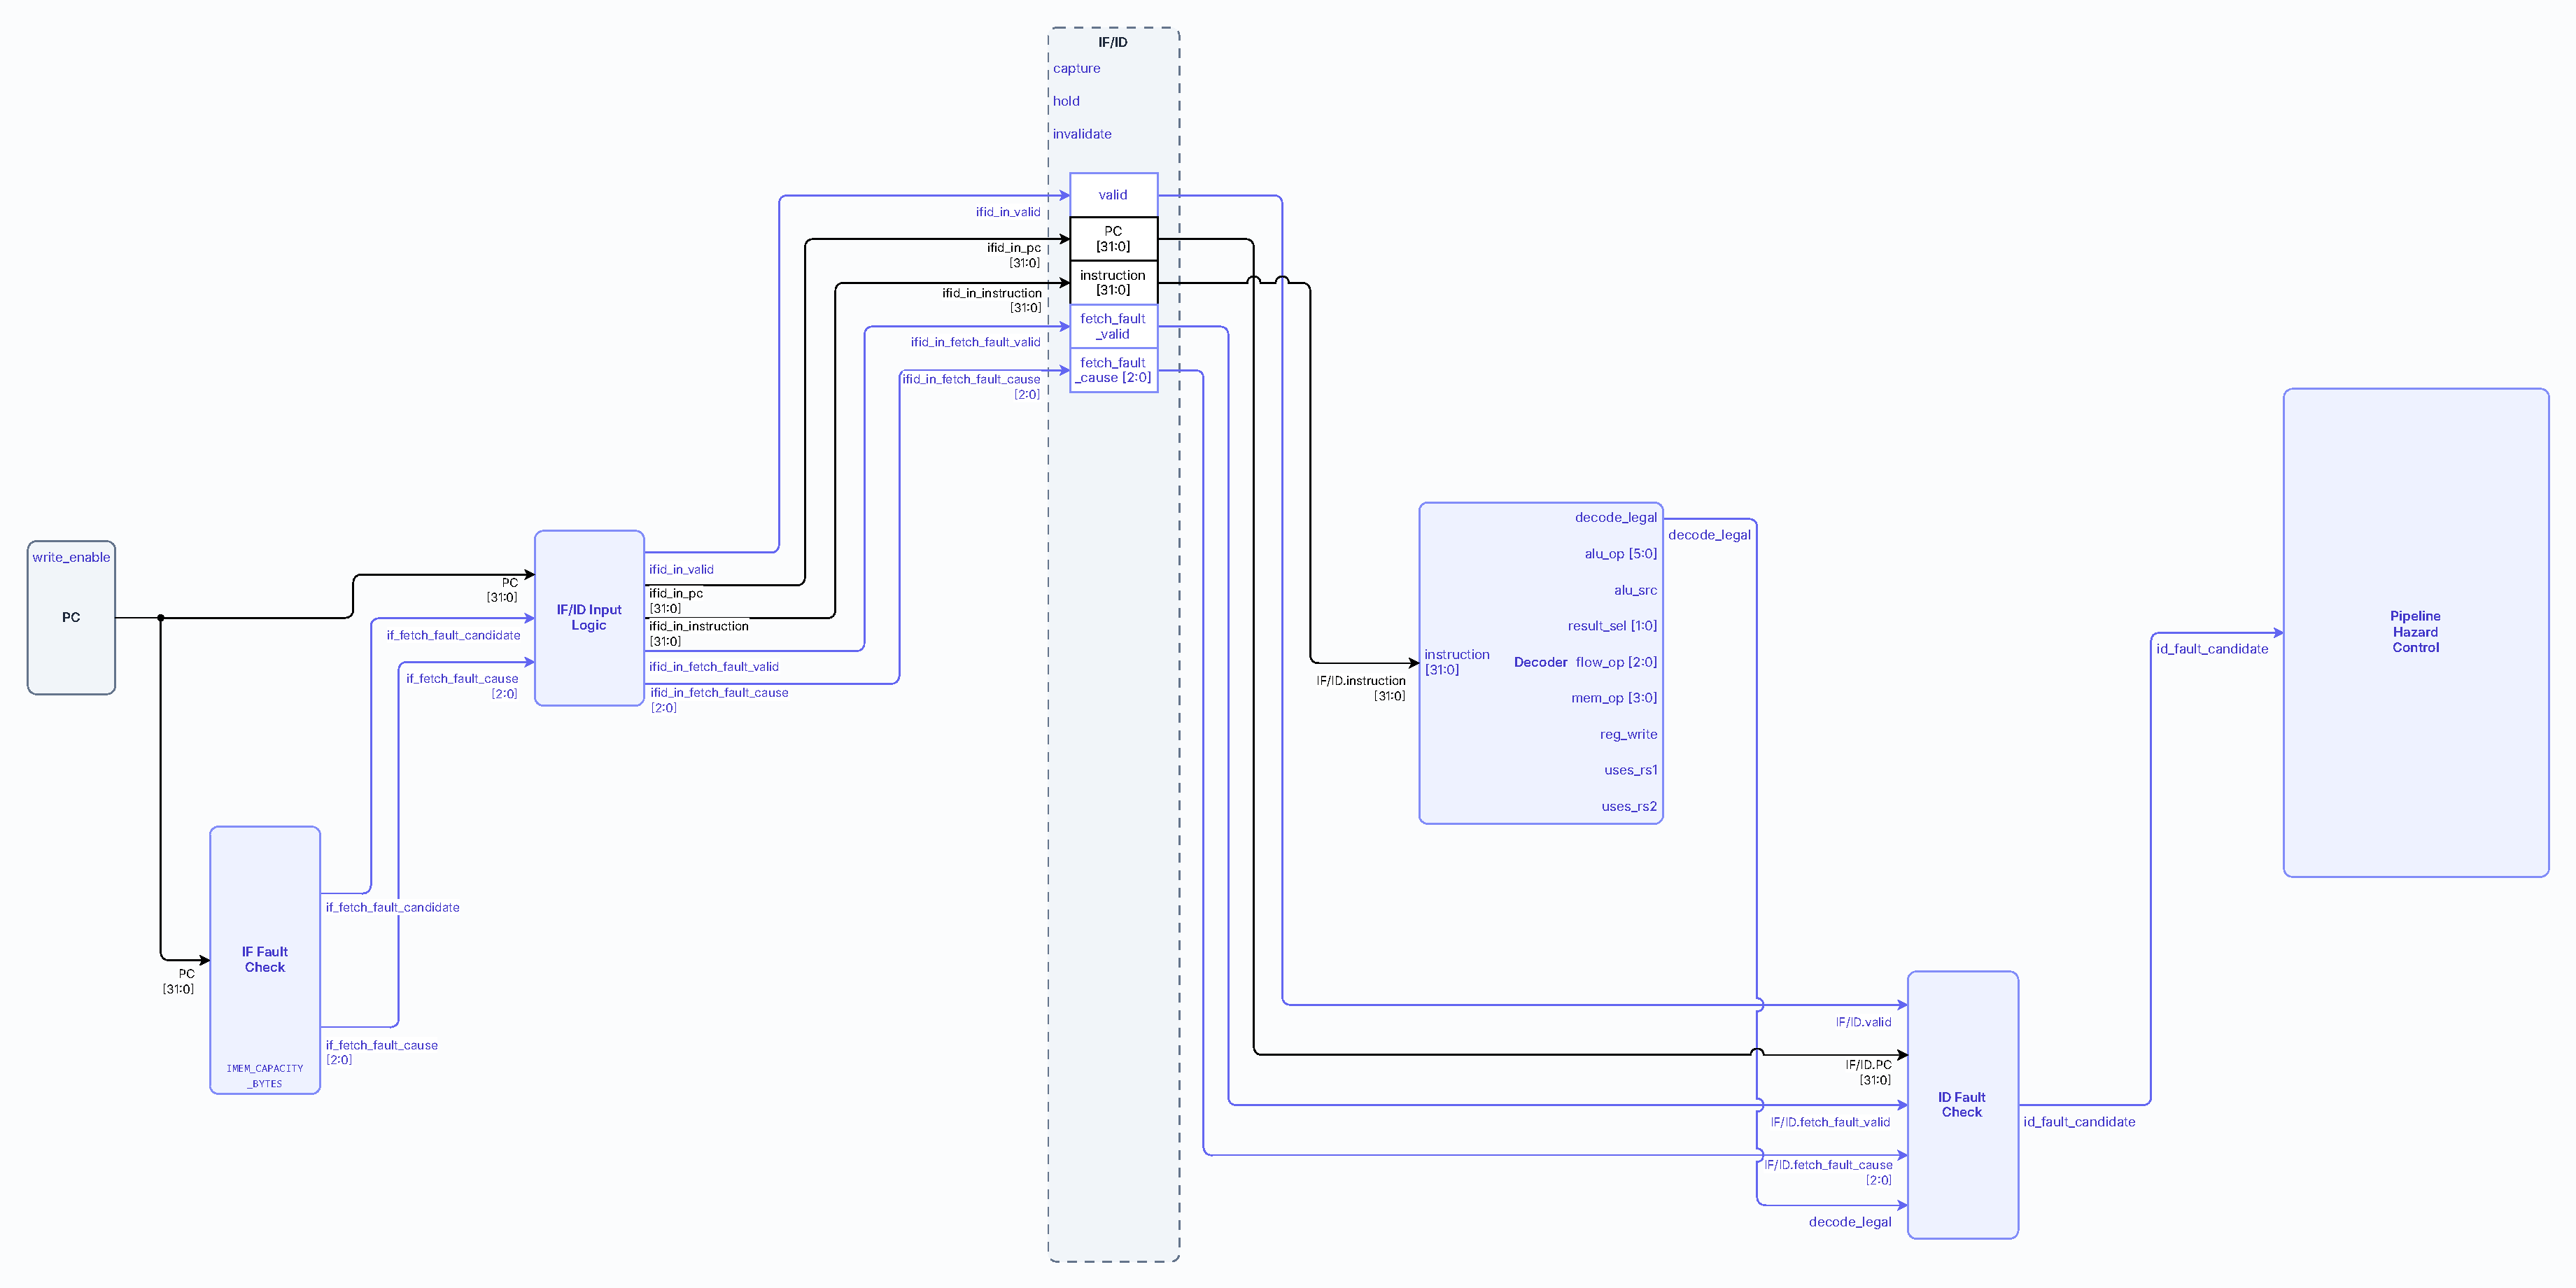
\includegraphics[width=0.95\textwidth]{fetch-fault.pdf}
  \caption{Recorrido del candidato de fault de fetch y su transporte por
  IF/ID.}
  \label{fig:fetch-fault}
\end{figure}
